\chapter{最优化}
\label{chap:optimization}

第~\ref{chap:mathematical-analysis}章说明了函数在一点附近怎样变化。本章要把这些局部信息
用于一个整体问题：在所有允许的参数中，怎样判断某个参数已经足够好，又怎样逐步找到它？
贯穿全章的对象是带正则项的最小二乘
\begin{equation}
  F(\bm{w})
  =
  \frac{1}{2n}\lVert \bm{X}\bm{w}-\bm{y}\rVert_2^2
  +\frac{\lambda}{2}\lVert\bm{w}\rVert_2^2,
  \qquad
  \bm{X}\in\mathbb{R}^{n\times d},\quad \lambda\geq 0,
  \label{eq:opt-regularized-least-squares}
\end{equation}
以及线性资源约束
\begin{equation}
  \bm{A}\bm{w}=\bm{b},\qquad
  \bm{G}\bm{w}\leq\bm{h}.
  \label{eq:opt-linear-resource-constraints}
\end{equation}
式~\eqref{eq:opt-regularized-least-squares}与第~\ref{chap:sets-functions-and-proofs}章的
式~\eqref{eq:prelim-regularized-least-squares}是同一个目标的矩阵写法。正则项限制参数
规模，约束则直接排除超出预算的候选；两者看似都在“限制模型”，却改变了不同的数学对象。

本章先说明解的存在与曲率如何决定局部信息的效力，再用约束、乘子、对偶和松弛建立
可核验的最优性证书；在认清目标与保证后，讨论光滑迭代、代理上界，以及非光滑项和不完整
梯度需要的更新方式。分块、多目标和双层问题不是
一条由旧到新的算法路线，而是三种不同的问题组织方式。读完本章，读者应能判断一个优化结论
依赖哪些条件，并能指出条件失效时究竟失去了存在性、全局性、唯一性还是收敛速度。

\section{目标、解与曲率}
\label{sec:opt-objectives-solutions-curvature}

求解算法之前，需要分清三件事：问题是否有解、怎样认出最优点，以及局部信息能否保证全局最优。
存在性主要依赖目标与可行域的闭合性质；凸性和其他曲率条件则决定驻点、解的唯一性与误差界。
这些是后面各种算法共用的前提，不是三种求解方法。

\subsection{问题设定与解的性质}
\label{sec:opt-problem-and-solutions}

\subsubsection{可行性、最优性与近似标准}

一个优化问题必须同时给出目标函数、变量和可行域。记
\[
  \min_{\bm{w}\in C}F(\bm{w}),\qquad
  C=\{\bm{w}\in\mathbb{R}^d:
  \bm{A}\bm{w}=\bm{b},\ \bm{G}\bm{w}\leq\bm{h}\}.
\]
若$C=\varnothing$，问题\term{不可行}（infeasible）；若$C\neq\varnothing$但
$\inf_{\bm{w}\in C}F(\bm{w})=-\infty$，问题\term{无下界}（unbounded below）。
只有可行且有有限下界，才值得继续问下确界是否由某个点达到。

\begin{definition}[全局解、局部解与无约束驻点]
\label{def:opt-solutions-stationarity}
设$C\subseteq\mathbb R^d$非空，$F:C\to\mathbb R$。\term{全局最优解}（global minimizer）$\bm{w}^{\star}\in C$满足
$F(\bm{w}^{\star})\leq F(\bm{w})$对所有$\bm{w}\in C$成立。\term{局部最优解}
（local minimizer）要求存在$r>0$，使该不等式对所有
$\bm w\in C\cap B(\bm w^\star,r)$成立。
无约束可微问题的\term{驻点}（stationary point）满足
$\nabla F(\bm{w})=\bm{0}$。驻点只是局部一阶变化消失，可能是极小点、极大点或
第~\ref{sec:analysis-second-order-curvature}节所说的微分鞍点。
\end{definition}
给定$\varepsilon>0$和可行候选$\widehat{\bm w}\in C$，若
\[
  F(\widehat{\bm{w}})-\inf_{\bm{w}\in C}F(\bm{w})\leq\varepsilon,
\]
就称$\widehat{\bm{w}}$为目标值意义下的$\varepsilon$近似解。对无约束可微问题，
另一种常见标准是
$\lVert\nabla F(\widehat{\bm{w}})\rVert_2\leq\varepsilon$；在没有额外曲率条件时，
这两种近似不能互换。一般约束问题的精确最优点也可能有非零梯度，此时应改用投影梯度、
可行方向导数或KKT残差等同时反映可行性与驻点性的标准。

\subsubsection{目标值、参数与预测误差}
\label{sec:opt-error-objects}

前面的目标值近似标准只比较目标与最优值之间的差距。评价同一个近似参数时，还可以关心它离某个参照参数多远，
或者它的预测发生了多大变化。这三个问题要分别选择误差对象。
下面暂取$C=\mathbb{R}^d$，不加资源约束，以式~\eqref{eq:opt-regularized-least-squares}为目标。
令$F^\star=\inf_{\bm{w}\in\mathbb{R}^d}F(\bm{w})$；若选定一个最小点
$\bm{w}^\star$，则
\[
  F(\widehat{\bm{w}})-F^\star,\qquad
  \lVert\widehat{\bm{w}}-\bm{w}^\star\rVert_2,\qquad
  \left(
    \frac{1}{n}\sum_{i=1}^{n}
    \bigl(
      \widehat{\bm{w}}^{\top}\bm{x}_i
      -(\bm{w}^\star)^{\top}\bm{x}_i
    \bigr)^2
  \right)^{1/2}
\]
分别是目标值误差、参数误差和在给定样本输入上的预测误差。最小点不唯一时，参数误差还
需要指定参照解，或改成到最小点集合的距离。三种误差衡量不同对象，彼此能否控制取决于
目标曲率、数据矩阵和参数化；一个误差较小不能无条件推出另两个也较小。

例如，在$n=1$、$\bm{x}_1=(1,0)^\top$、$y_1=0$、$\lambda=0$时，
目标函数为$F(w_1,w_2)=w_1^2/2$。参照解$(0,0)$与参数$(0,100)$的目标值都为$0$，
在这个样本输入上的预测也相同，参数距离却是$100$。差别来自目标和当前观测都没有约束
第二个坐标；并不是把目标误差算得更精确就能补回这项信息。

\subsubsection{解的存在、唯一与稳定性}

若$C\subseteq\mathbb{R}^d$非空且紧，$F:C\to\mathbb{R}$连续，则
定理~\ref{thm:analysis-extreme-value}保证$F$在$C$上达到全局最小值。这里直接复用
第~\ref{chap:mathematical-analysis}章的极值存在结论。

可行域不紧时，目标本身也可能阻止最小化序列逃向无穷远。
\begin{definition}[强制性与下半连续性]
\label{def:opt-coercive-lower-semicontinuous}
设$C\subseteq\mathbb R^d$，$F:C\to(-\infty,+\infty]$。若沿$C$中的任意序列，
$\lVert\bm{w}\rVert_2\to\infty$时$F(\bm{w})\to\infty$，称$F$是
\term{强制的}（coercive）。$F$在$C$上\term{下半连续}
（lower semicontinuous）要求对每个收敛序列
$\bm{w}^{(k)}\to\bm{w}$都有
\[
  F(\bm{w})\leq\liminf_{k\to\infty}F(\bm{w}^{(k)}).
\]
其中序列与极限点均属于$C$。
\end{definition}
连续性并不是存在性证明所需的最弱条件。下半连续性允许函数值在极限点向下跳，
却不允许极限点的函数值突然高于邻近值。等价地，每个
下水平集$\{\bm{w}\in C:F(\bm{w})\leq a\}$在$C$的相对拓扑中都是闭集。

设$C$非空且闭，$F:C\to(-\infty,+\infty]$下半连续、强制，并且不恒为
$+\infty$且从不取$-\infty$。取$\bar{\bm{w}}\in C$使
$F(\bar{\bm{w}})<+\infty$，再把最小化序列限制到下水平集
\[
  K=\{\bm{w}\in C:F(\bm{w})\leq F(\bar{\bm{w}})\}.
\]
若$\inf_C F=F(\bar{\bm{w}})$，则$\bar{\bm{w}}$已经是最小点；否则
$\inf_C F<F(\bar{\bm{w}})$，任一最小化序列从某项起都落入$K$，可以只保留这段尾序列。
强制性使$K$有界，下半连续性与$C$的闭性使$K$闭，故$K$在有限维空间中紧。该尾序列
有子列收敛到$\bm{w}^{\star}\in K$，而下半连续性给出
$F(\bm{w}^{\star})\leq\liminf_kF(\bm{w}^{(k)})=\inf_C F$。因此下确界达到。
这个证明也指出各条件的职责：强制性阻止序列逃向无穷远，闭性保留可行极限，下半连续性
把目标值比较传到极限点。
当$\lambda>0$时，式~\eqref{eq:opt-regularized-least-squares}满足
$F(\bm{w})\geq\lambda\lVert\bm{w}\rVert_2^2/2$，所以即使可行域无界也不会沿参数
无穷大的方向降低目标。

存在不等于唯一。若$\lambda=0$且$\bm{X}$有非零零空间向量$\bm{v}$，那么
$F(\bm{w}+t\bm{v})=F(\bm{w})$，最小点可能形成一条直线。即使唯一，数值问题也可能
非常敏感。例如令$0<\epsilon\ll1$并考虑
\[
  f_b(w_1,w_2)=\frac12(\epsilon w_1^2+w_2^2)-bw_1.
\]
它对每个$b$都有唯一最小点$(b/\epsilon,0)$，但$b$改变$\Delta b$会使第一坐标改变
$\Delta b/\epsilon$。更一般的二次目标具有如下曲率矩阵：
\[
  \bm{H}=\frac{1}{n}\bm{X}^{\top}\bm{X}+\lambda\bm{I}
\]
当$\bm{H}\succ\bm{0}$时，若线性项受到加性扰动$\delta\bm{g}$，相应解变化满足
\[
  \lVert\delta\bm{w}\rVert_2
  \leq
  \frac{1}{\lambda_{\min}(\bm{H})}
  \lVert\delta\bm{g}\rVert_2.
\]
因此$1/\lambda_{\min}(\bm{H})$控制固定尺度加性扰动的绝对放大；经过目标和变量尺度
归一化后，条件数
$\kappa(\bm{H})=\lambda_{\max}(\bm{H})/\lambda_{\min}(\bm{H})$
才刻画相对病态程度。例如$\bm{H}=\epsilon\bm{I}$的条件数为$1$，但绝对扰动仍会被
放大$1/\epsilon$倍。唯一性回答“解有几个”，敏感性还取决于所采用的扰动尺度，
不能只由唯一性或条件数笼统判断。

\subsection{凸集与凸函数}
\label{sec:opt-convexity}

\subsubsection{线段、曲率与全局下界}

约束只告诉我们哪些点允许使用；还要问两个可行点之间能否连续移动而始终可行。
\begin{definition}[凸集与凸函数]
\label{def:opt-convex-set-function}
集合$C\subseteq\mathbb R^d$为\term{凸集}（convex set），是指对任意
$\bm{u},\bm{v}\in C$和$\theta\in[0,1]$，
$\theta\bm{u}+(1-\theta)\bm{v}\in C$。线性等式、线性不等式和范数球的解集都是凸集，
它们的交集仍为凸集，所以式~\eqref{eq:opt-linear-resource-constraints}定义凸可行域。

定义在凸集$C$上的函数$f:C\to\mathbb R$若对任意$\bm u,\bm v\in C$和$\theta\in[0,1]$满足
\begin{equation}
  f(\theta\bm{u}+(1-\theta)\bm{v})
  \leq
  \theta f(\bm{u})+(1-\theta)f(\bm{v}),
  \label{eq:opt-convex-function}
\end{equation}
就称为\term{凸函数}（convex function）。若$-f$凸，则称$f$凹。
\end{definition}
凸函数的函数图像位于任意弦段下方，因此局部低点
不会被更远处的谷底击败\scite{math-boyd2004convex}

\begin{theorem}[凸函数的一阶与二阶判据]
\label{thm:opt-convexity-criteria}
设$C$为开凸集。可微函数$f:C\to\mathbb{R}$凸，当且仅当对任意
$\bm{u},\bm{v}\in C$，
\begin{equation}
  f(\bm{v})\geq f(\bm{u})
  +\langle\nabla f(\bm{u}),\bm{v}-\bm{u}\rangle.
  \label{eq:opt-first-order-convexity}
\end{equation}
若$f$二阶可微，则这又等价于
$\nabla^2f(\bm{w})\succeq\bm{0}$对所有$\bm{w}\in C$成立。
\end{theorem}

\begin{proof}
若$f$凸，令$\phi(t)=f(\bm{u}+t(\bm{v}-\bm{u}))$。由凸性，
$[\phi(t)-\phi(0)]/t\leq\phi(1)-\phi(0)$。令$t\downarrow0$便得
式~\eqref{eq:opt-first-order-convexity}。反过来，令
$\bm{z}=\theta\bm{u}+(1-\theta)\bm{v}$，分别把一阶不等式用于
$(\bm{z},\bm{u})$和$(\bm{z},\bm{v})$，乘以$\theta$与$1-\theta$后相加，
线性项抵消，得到式~\eqref{eq:opt-convex-function}。

若$f$凸，把一阶判据用于$\bm{w}$与$\bm{w}+t\bm{v}$，再对$t$求二阶局部极限，
得到$\bm{v}^{\top}\nabla^2f(\bm{w})\bm{v}\geq0$。反之，沿任意线段定义
$\phi(t)$，则
$\phi''(t)=(\bm{v}-\bm{u})^{\top}\nabla^2f(\bm{u}+t(\bm{v}-\bm{u}))
(\bm{v}-\bm{u})\geq0$，一元函数$\phi$凸，故$f$凸。
\end{proof}

反复应用二点凸性可得\term{Jensen不等式}（Jensen's inequality）。若
$\alpha_i\geq0$且$\sum_i\alpha_i=1$，则
\begin{equation}
  f\left(\sum_{i=1}^m\alpha_i\bm{w}_i\right)
  \leq\sum_{i=1}^m\alpha_i f(\bm{w}_i).
  \label{eq:opt-jensen}
\end{equation}
归纳步骤把前$m-1$个点先归一化为一个加权平均，再与第$m$个点应用二点凸性。
这个证明也说明非负和归一化不是装饰条件；允许负权重后，组合点可能落到凸包之外，
因而不能再由凸性保证Jensen不等式。

凸性还把最优性变成可核验的一阶条件。若$f$可微且凸，则
$\nabla f(\bm{w}^{\star})=\bm{0}$代入式~\eqref{eq:opt-first-order-convexity}
便得$f(\bm{v})\geq f(\bm{w}^{\star})$。因此凸问题的驻点是全局最小点。
图~\ref{fig:opt-convex-chord-tangent}同时画出这两侧的界。弦在图像上方，源于二点凸组合；
切线在图像下方，源于可微凸函数的一阶判据。二者夹住函数，却来自不同的比较对象，
不能把某点处的切线误当作连接两个函数值的弦。
\begin{figure}[htbp]
 \centering
 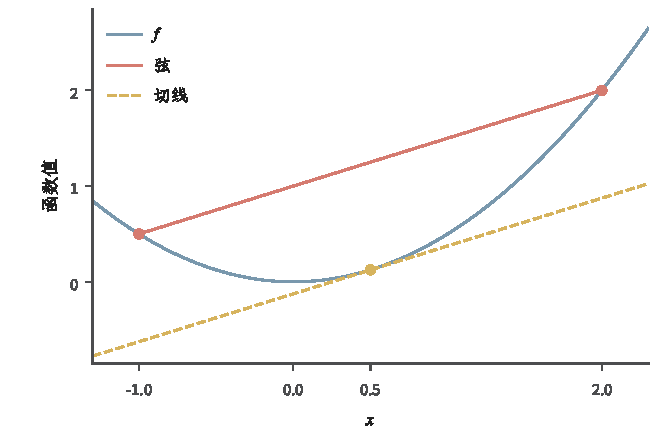
\includegraphics[width=\linewidth]{figures/math-preparation/reader-revision-analysis/optimization-convex-chord-tangent.pdf}
 \caption{$f(x)=x^2/2$的弦与切线。蓝线为函数，红线连接$u=-1$与$v=2$的函数值，
 在这两个输入之间给出弦上界；黄虚线是在$x_0=1/2$处的一阶仿射下界，适用于整个实线。
 红线的上界只在其端点之间使用，切线下界来自凸性。图为解析教学示例。}
 \label{fig:opt-convex-chord-tangent}
\end{figure}


\begin{definition}[严格凸函数]
\label{def:opt-strict-convexity}
设$C$凸，$f:C\to\mathbb R$。若式~\eqref{eq:opt-convex-function}对所有
$\bm u\neq\bm v$及$0<\theta<1$严格成立，则称$f$严格凸。
\end{definition}
严格凸保证最小点至多一个，却不给统一曲率下界。强凸性则要求弦段与函数之间至少留出一个与距离平方成比例的间隔。
这个定义可以用于非光滑正则项，也可以使用欧氏范数以外的范数。

\begin{definition}[相对于范数的强凸性]
\label{def:opt-strong-convexity}
设$C$是实赋范空间中的凸集，$f:C\to\mathbb{R}$，$\mu>0$。若对任意
$\bm{u},\bm{v}\in C$和$\theta\in[0,1]$都有
\begin{equation}
 f(\theta\bm{u}+(1-\theta)\bm{v})
 \leq\theta f(\bm{u})+(1-\theta)f(\bm{v})
 -\frac{\mu}{2}\theta(1-\theta)\lVert\bm{u}-\bm{v}\rVert^2,
 \label{eq:opt-norm-strong-convexity}
\end{equation}
则称$f$相对于$\lVert\cdot\rVert$是\term{$\mu$强凸}（$\mu$-strongly convex）的。
\end{definition}

在欧氏空间的开凸集上，若$f$可微，强凸性等价于一阶下界
\begin{equation}
  f(\bm{v})\geq f(\bm{u})+
  \langle\nabla f(\bm{u}),\bm{v}-\bm{u}\rangle
  +\frac{\mu}{2}\lVert\bm{v}-\bm{u}\rVert_2^2.
  \label{eq:opt-first-order-strong-convexity}
\end{equation}
可用定理~\ref{thm:opt-convexity-criteria}对
$f(\bm{w})-\mu\lVert\bm{w}\rVert_2^2/2$应用凸性判据得到这一等价关系；若$f$二阶可微，
它又等价于$\nabla^2f(\bm{w})\succeq\mu\bm{I}$。一般范数的平方未必是欧氏二次型，
因此不能把这一Hessian写法直接当作所有范数下的定义。
例如$|x|+\mu x^2/2$虽在$0$处不可微，仍相对于绝对值范数$\mu$强凸：绝对值部分满足
凸性，二次部分恰好提供式~\eqref{eq:opt-norm-strong-convexity}中的距离平方间隔。

一阶算法还需要防止梯度随位移过快改变。
\begin{definition}[欧氏梯度光滑性]
\label{def:opt-smoothness}
设$C\subseteq\mathbb R^d$开且凸，$f:C\to\mathbb R$可微，$L\geq0$有限。
$f$为\term{$L$光滑}（$L$-smooth），是指对任意$\bm u,\bm v\in C$，梯度满足
$\lVert\nabla f(\bm{u})-\nabla f(\bm{v})\rVert_2
\leq L\lVert\bm{u}-\bm{v}\rVert_2$。
\end{definition}
这里对梯度使用同一Lipschitz常数。强凸给下曲率，光滑给上曲率；$x^4$严格凸但
不在全实线上强凸，也不在全实线上具有有限的光滑常数。

\subsection{较弱曲率与非凸结构}
\label{sec:opt-weaker-curvature}

凸性同时约束所有线段上的函数值，有时比具体求解所需的条件更强。
下面分开讨论两种放宽：弱凸允许负曲率但限制其大小，PL条件直接把梯度大小与目标差联系起来。
它们服务于不同推导，不应把名称看成从凸到非凸的单一强弱序列。

\subsubsection{弱凸与补足曲率}

强凸同时控制函数形状和误差。实际目标可能不凸，却仍有足够结构支持算法分析。
\begin{definition}[欧氏空间中的弱凸性]
\label{def:opt-weak-convexity}
设$f:\mathbb{R}^d\to\mathbb{R}\cup\{+\infty\}$是适当函数，即不恒为$+\infty$，
且$\rho\geq0$。若
$\bm{w}\mapsto f(\bm{w})+\rho\lVert\bm{w}\rVert_2^2/2$是凸函数，
则称$f$是\term{$\rho$弱凸}（$\rho$-weakly convex）的。取值$+\infty$可以用来表示不可行点。
\end{definition}
若$f$在开凸定义域上二阶可微，这等价于
$\nabla^2f(\bm{w})\succeq-\rho\bm{I}$：负曲率可以存在，但有统一下界。
当$\rho>0$且$0<\eta<1/\rho$时，对任意中心$\bm{z}$，邻近子问题的目标
\[
  f(\bm{w})+\frac{1}{2\eta}\lVert\bm{w}-\bm{z}\rVert_2^2
\]
是$(1/\eta-\rho)$强凸函数；若$\rho=0$，任意$\eta>0$都具有同样的补足曲率作用。
这正是弱凸性与第~\ref{sec:opt-nonsmooth-proximal}节邻近方法的联系。补入二次曲率
只让这个子问题更易控制，并没有把原函数变成凸函数；弱凸目标仍可有局部极小点和鞍点，
也不保证求得原问题的全局最优解。

例如$f(x)=\cos x$的二阶导数是$-\cos x\geq-1$，所以它是$1$弱凸的，
但仍有无穷多个局部低点。弱凸性限制谷之间最坏的负曲率，并未消除这些谷。
若在当前位置附近加上足够大的二次惩罚，邻近子问题会得到唯一解；改变当前位置后，
所解的却是另一个邻近子问题，不能据此声称原函数只有一个最小点。

\subsubsection{Polyak--Łojasiewicz条件}

\term{Polyak--Łojasiewicz条件}（PL condition）不约束函数图像必须凸，而用梯度大小控制
距离最优值还有多少差距。
\begin{definition}[Polyak--Łojasiewicz条件]
\label{def:opt-pl-condition}
设$f:\mathbb{R}^d\to\mathbb{R}$可微，$f^\star=\inf_{\bm{w}}f(\bm{w})> -\infty$。
若存在$\mu>0$，使任意$\bm{w}$满足
\begin{equation}
  \frac{1}{2}\lVert\nabla f(\bm{w})\rVert_2^2
  \geq \mu\bigl(f(\bm{w})-f^{\star}\bigr),
  \qquad \mu>0.
  \label{eq:opt-pl-condition}
\end{equation}
则称$f$满足常数为$\mu$的PL条件。
\end{definition}
该条件把小梯度与小目标误差联系起来。强凸可推出PL条件：对$\mu$强凸可微函数，把强凸
下界右侧关于$\bm{v}$最小化，得到
\[
  f^\star\geq
  f(\bm{w})-\frac{1}{2\mu}\lVert\nabla f(\bm{w})\rVert_2^2,
\]
移项正是式~\eqref{eq:opt-pl-condition}。这个推导使用全局强凸下界；只有局部Hessian
正定时，不能直接得到全域PL条件。反过来，PL函数可以有多个最小点。

同一个低维族能显示这些性质各自控制什么。令
\[
  f_a(x_1,x_2)=\frac12(x_1+x_2)^2+\frac{a}{2}(x_1-x_2)^2.
\]
当$a>0$时函数强凸；$a=0$时它凸且满足PL条件，但整条直线$x_1+x_2=0$都是最小点；
$a<0$时函数弱凸却无下界。若限制在紧可行域上，$a<0$时仍有最小点，但驻点
$(0,0)$可能是鞍点。这个例子说明弱凸、PL和强凸不是一条简单的强弱链：弱凸限制最坏负
曲率，PL控制梯度与目标误差，强凸还控制参数距离与唯一性。

PL条件也确实可以出现在非凸函数中。考虑
\[
  f(x,y)=x^2+2\sin^2x.
\]
它与$y$无关，因而最小点不唯一。其一阶导数为
$\partial f/\partial x=2(x+\sin 2x)$；当$x>0$时，若$x\leq1$则两项均非负，
若$x>1$则$x+\sin2x\geq x-1>0$，负半轴由奇对称性处理，所以导数只在$x=0$时
为零。比值
\[
  R(x)=\frac{\lVert\nabla f(x,y)\rVert_2^2}{2f(x,y)}
\]
在$x\neq0$时为正，并且$x\to0$时趋于$6$，$|x|\to\infty$时趋于$2$。
把两端之外的剩余区域限制为紧集，连续函数$R$在其中有正下界，故某个$\mu>0$使
式~\eqref{eq:opt-pl-condition}成立。另一方面，
$\partial^2 f/\partial x^2=2+4\cos2x$在某些点为负，所以$f$并不凸；该二阶导数
下界为$-2$、绝对值上界为$6$，又说明它同时是$2$弱凸且$6$光滑。这个例子不能推出
所有弱凸函数都满足PL条件，它只表明非凸性本身不排斥目标值的梯度控制。

式~\eqref{eq:opt-regularized-least-squares}的Hessian矩阵为
$\bm{X}^{\top}\bm{X}/n+\lambda\bm{I}$。当$\lambda>0$时，正则项把所有缺失曲率的
方向至少抬高到$\lambda$，因而目标$\lambda$强凸。若$\lambda=0$且$\bm{X}$不满列秩，
驻点仍是全局最优点，但解不唯一；若目标再加入非凸项，驻点甚至不再保证局部最小。

\begin{table*}[htbp]
 \centering\small
 \begin{tabularx}{\linewidth}{@{}lXX@{}}
 \toprule
 条件 & 直接控制什么 & 单凭该条件不能得到什么\\
 \midrule
 凸性 & 全部线段上的弦上界；局部最小点也是全局最小点 & 最小点存在、唯一或统一收敛速率\\
 严格凸性 & 非平凡线段上的严格不等式；最小点至多一个 & 一致正曲率下界，例如$x^4$在原点曲率为零\\
 强凸性 & 函数值相对切平面的二次增长（可微情形） & 梯度光滑性，例如$|x|+\mu x^2/2$仍有尖点\\
 弱凸性 & 最坏负曲率的统一下界 & 驻点全局最优或最小点唯一\\
 PL条件 & 梯度大小控制目标值差 & 凸性或参数解的唯一性\\
 \bottomrule
 \end{tabularx}
 \caption{曲率条件的职责比较。各行针对不同性质，不能排成一条从“弱”到“强”的完整等级。}
 \label{tab:opt-curvature-conditions}
\end{table*}

\section{约束、对偶与最优性证书}
\label{sec:opt-constraints-duality-certificates}

前节的局部驻点标准允许考察任意方向；有资源约束时，降低目标的方向可能不可行。
乘子把可行方向的限制纳入一阶条件，对偶把这些限制转换为目标的下界，松弛则让难以直接求解的问题也能得到可计算的界。
三者共同回答：一个候选解是否可行，以及还可能改善多少。

\subsection{凸几何与仿射下界}
\label{sec:opt-affine-certificates}
把不可行或次优转为可核验的线性不等式，需要先说明分离与支撑；
再把同样的仿射下界语言用于函数，就能理解共轭与对偶中的界来自哪里。

\subsubsection{最近点与线性分离}

\begin{theorem}[闭凸集外一点的严格分离]
\label{thm:opt-projection-separation}
设$C\subseteq\mathbb{R}^d$非空、闭且凸，$\bm{z}\notin C$。则存在
$\bm{a}\neq\bm{0}$和$c\in\mathbb{R}$，使
\[
  \langle\bm{a},\bm{x}\rangle\leq c
  <\langle\bm{a},\bm{z}\rangle
  \quad\text{对所有 }\bm{x}\in C.
\]
\end{theorem}

\begin{proof}
先证明所需最近点的存在性与唯一性。任取$\bm{x}_0\in C$并令
$R=\lVert\bm{z}-\bm{x}_0\rVert_2$。集合
\[
  C_R=C\cap\{\bm{x}:\lVert\bm{z}-\bm{x}\rVert_2\leq R\}
\]
非空、闭且有界，因而在有限维空间中紧。连续函数
$\lVert\bm{z}-\bm{x}\rVert_2^2$在$C_R$上达到最小值；球外各点到$\bm{z}$的
距离大于$R$，而$\bm{x}_0$的距离等于$R$，所以该最小点也是$C$上的最近点。
若$\bm{p}_1,\bm{p}_2$都是最近点，最近距离为$\delta$，则凸性保证其中点属于$C$，且
\[
  \left\lVert\bm{z}-\frac{\bm{p}_1+\bm{p}_2}{2}\right\rVert_2^2
  =
  \frac12\lVert\bm{z}-\bm{p}_1\rVert_2^2
  +\frac12\lVert\bm{z}-\bm{p}_2\rVert_2^2
  -\frac14\lVert\bm{p}_1-\bm{p}_2\rVert_2^2.
\]
当$\bm{p}_1\neq\bm{p}_2$时，右端严格小于$\delta^2$，与最近距离的定义矛盾，故最近点
唯一，记为$\bm{p}$。

对任意$\bm{x}\in C$，
$\bm{p}+t(\bm{x}-\bm{p})\in C$。函数
$q(t)=\lVert\bm{z}-\bm{p}-t(\bm{x}-\bm{p})\rVert_2^2$在$t=0$
处右导数非负，所以
$\langle\bm{z}-\bm{p},\bm{x}-\bm{p}\rangle\leq0$。取
$\bm{a}=\bm{z}-\bm{p}$和$c=\langle\bm{a},\bm{p}\rangle$，则
$\langle\bm{a},\bm{x}\rangle\leq c$，而
$\langle\bm{a},\bm{z}\rangle=c+\lVert\bm{a}\rVert_2^2>c$。
\end{proof}

\begin{definition}[支撑超平面与凸锥]
\label{def:opt-supporting-hyperplane-cone}
设$C\subseteq\mathbb R^d$非空，$\bm a\neq0$。若$C$全部位于
$\{\bm x:\langle\bm a,\bm x\rangle\leq c\}$，并且至少有一点取等号，
则等号超平面称为$C$的\term{支撑超平面}（supporting hyperplane）。
非空集合$K$若对所有$\bm u,\bm v\in K$、$\alpha,\beta\geq0$都有
$\alpha\bm u+\beta\bm v\in K$，称为凸锥。
\end{definition}
具体地说，若$\bm{p}$位于闭凸集$C$的边界，可取一列集外点
$\bm{z}^{(k)}\to\bm{p}$，对每个点应用严格分离并把法向量归一化。单位球的紧性给出
收敛子列，极限法向量$\bm{a}\neq\bm{0}$满足
$\langle\bm{a},\bm{x}\rangle\leq\langle\bm{a},\bm{p}\rangle$对所有
$\bm{x}\in C$成立。这说明边界处至少有一个支撑方向，但边界有棱角时法向量未必唯一。
分离把“点不属于集合”转化为一个线性不等式证书，但它本身不自动给出一般凸问题的强对偶；
还需要闭性或约束资格条件。

对称矩阵集合中的\term{半正定锥}（positive semidefinite cone）
\[
  \mathbb{S}_+^d=\{\bm{M}=\bm{M}^{\top}:
  \bm{v}^{\top}\bm{M}\bm{v}\geq0,\ \forall\bm{v}\}
\]
是凸锥，因为非负线性组合仍保持二次型非负。它也是闭集：若
$\bm{M}^{(k)}\to\bm{M}$且每个$\bm{M}^{(k)}\succeq\bm{0}$，则对任意固定
$\bm{v}$都有
$\bm{v}^{\top}\bm{M}\bm{v}
=\lim_k\bm{v}^{\top}\bm{M}^{(k)}\bm{v}\geq0$。
线性规划的非负正交锥和半正定规划的矩阵约束直接定义凸可行域；标准凸二次规划中的
半正定曲率矩阵则保证目标凸。三者共享的是凸目标与凸可行域的语言。若要进一步统一成
带线性目标的锥规划，还需引入辅助变量，对二次目标作上图或锥提升。

\subsubsection{凸共轭与双共轭}

分离用仿射函数区分一个点与可行集合。对目标函数，也可以收集所有仿射下界：
固定斜率后找最紧的截距，再比较所有斜率能否重建原函数。凸共轭承担这一步。
\begin{definition}[适当函数、有效定义域与约束指标]
\label{def:opt-proper-domain-indicator}
函数$f:\mathbb R^d\to\mathbb R\cup\{+\infty\}$若不恒为$+\infty$，称为适当函数；
它从不取$-\infty$。其\term{有效定义域}（effective domain）为
$\operatorname{dom}f=\{\bm x:f(\bm x)<+\infty\}$。
集合$C$的扩展实值指标函数为$\iota_C(\bm x)=0$（$\bm x\in C$），在其余点取$+\infty$。
\end{definition}
这个指标不是第~\ref{chap:sets-functions-and-proofs}章取$0/1$的指示函数。
它把不允许的点排除出最小化，而不只是给集合成员作标记。
对扩展实值目标，式~\eqref{eq:opt-convex-function}在有限取值的点上检验，
并要求有效定义域凸；这避免在端点权重为零时操作$0\cdot(+\infty)$。
上图集$\operatorname{epi}f=\{(\bm x,r)\in\mathbb R^{d+1}:r\geq f(\bm x)\}$
记录图像以上的全部点；它凸与$f$凸等价，闭与$f$下半连续等价。
\begin{definition}[凸共轭与双共轭]
\label{def:opt-conjugate}
给定适当函数$f:\mathbb R^d\to\mathbb R\cup\{+\infty\}$，其\term{凸共轭}
（convex conjugate）定义为
\begin{equation}
 f^*(\bm y)=\sup_{\bm x\in\mathbb R^d}
            \{\langle\bm y,\bm x\rangle-f(\bm x)\},
 \qquad
 f^{**}(\bm x)=\sup_{\bm y\in\mathbb R^d}
            \{\langle\bm y,\bm x\rangle-f^*(\bm y)\}.
 \label{eq:opt-conjugate-biconjugate}
\end{equation}
两个上确界都在整个$\mathbb R^d$上取。$f^*$允许取$+\infty$；若$f^*\equiv+\infty$，
则$f^{**}\equiv-\infty$，否则$f^{**}$不取$-\infty$，但仍可能取$+\infty$。
\end{definition}
这里$f(\bm x)=+\infty$的点不贡献有限共轭候选。固定斜率$\bm y$时，$f^*(\bm y)$是
让$\langle\bm y,\bm x\rangle-f^*(\bm y)$在全域不超过$f$所需的最小截距修正。
没有任何仿射下界时，这个修正对每个斜率都为无穷。例如$f(x)=-x^2$满足
$f^*(y)=\sup_x\{yx+x^2\}=+\infty$，双共轭因而恒为$-\infty$；适当性本身不能排除这一情形。
由定义立即有\term{Fenchel--Young不等式}
\[
 f(\bm x)+f^*(\bm y)\geq\langle\bm y,\bm x\rangle,
\]
以及$f^{**}\leq f$。共轭是仿射函数族的上确界，因而凸且下半连续；它并非简单把
函数图像交换横纵坐标，也不要求每个上确界都由有限斜率达到。

\begin{theorem}[有限维Fenchel--Moreau定理]
\label{thm:opt-fenchel-moreau}
设$f:\mathbb R^d\to\mathbb R\cup\{+\infty\}$适当、下半连续且凸。
则$f^{**}=f$在全部$\mathbb R^d$上成立，包括$f(\bm x)=+\infty$的点。
因此$f$恰好是全部连续仿射下界的逐点上确界。
\end{theorem}

\begin{proof}
上图集$\operatorname{epi}f=\{(\bm x,r):r\geq f(\bm x)\}$非空、闭且凸。
任取$\bm x_0\in\operatorname{dom}f$及$t_0<f(\bm x_0)$，对上图与其外一点
$(\bm x_0,t_0)$使用定理~\ref{thm:opt-projection-separation}，得到
\[
 \langle\bm a,\bm x_0\rangle+b t_0<c
 \leq\langle\bm a,\bm z\rangle+b r
 \quad\text{对所有 }(\bm z,r)\in\operatorname{epi}f.
\]
上图沿$r$向上无界，故$b\geq0$；若$b=0$，取
$(\bm z,r)=(\bm x_0,f(\bm x_0))$便矛盾，所以$b>0$。
重排得到一个全域仿射下界$\ell_0(\bm z)=\langle\bm p_0,\bm z\rangle-\beta_0\leq f(\bm z)$。
这也保证$f^*(\bm p_0)$有限。

现任取$\bm x$和实数$t<f(\bm x)$，再次严格分离$(\bm x,t)$与上图。
若所得竖直系数$b>0$，立即得到一个仿射下界$\ell$，满足$\ell(\bm x)>t$。
若$b=0$，分离不等式为$\langle\bm a,\bm x\rangle<c\leq\langle\bm a,\bm z\rangle$。
将它与$\varepsilon(r-\ell_0(\bm z))\geq0$相加，得到
\[
 \langle\bm a-\varepsilon\bm p_0,\bm z\rangle+\varepsilon r
 \geq c-\varepsilon\beta_0.
\]
取足够小的$\varepsilon>0$，在$(\bm x,t)$处仍为严格反向不等式，因为原来的分离
间隙为正。新的竖直系数为$\varepsilon>0$，因此仍得到$\ell\leq f$且$\ell(\bm x)>t$。

将这一仿射下界写为$\ell(\bm z)=\langle\bm y,\bm z\rangle-\beta$，有
$f^*(\bm y)\leq\beta$，所以
$f^{**}(\bm x)\geq\langle\bm y,\bm x\rangle-f^*(\bm y)
\geq\ell(\bm x)>t$。
若$f(\bm x)$有限，令$t\uparrow f(\bm x)$；若$f(\bm x)=+\infty$，让$t$任意增大，
两种情形均得$f^{**}(\bm x)\geq f(\bm x)$。结合反向不等式即得结论。
\end{proof}

例如$f(x)=x^2/2$的共轭仍是$y^2/2$，因为$x=y$达到上确界。
若$f=\iota_{[0,1]}$为闭区间指标函数，则$f^*(y)=\max\{0,y\}$，双共轭恢复区间内
的零值和区间外的$+\infty$。闭性不能省略：对开区间指标$f=\iota_{(0,1)}$，共轭仍为
$\max\{0,y\}$，但双共轭成为$\iota_{[0,1]}$，在两个端点补上零值。
仿射下界无法区分一个边界点与从内部趋近的极限，下半连续性正是排除这种缺口的条件。

函数等于双共轭也不保证边界处有有限的最优斜率。例如闭凸函数
$f(x)=-\sqrt{x}$对$x\geq0$定义，负半轴取$+\infty$。在$x=0$，有限次梯度$y$若存在，
必须满足$-\sqrt{x}\geq yx$对所有$x>0$成立，即$y\leq-1/\sqrt{x}$，这是不可能的。
$f^{**}(0)=f(0)=0$仍成立，但只能由一列仿射下界逼近，不能声称共轭上确界在某个有限
$y$处达到。由双共轭推导对偶表达时，值相等与最优乘子存在必须分别证明。

\subsection{约束与拉格朗日乘子}
\label{sec:opt-kkt}

\subsubsection{可行方向与KKT条件}

资源约束使最优点处的目标梯度不必为零，因为可行方向受到限制。对
\[
  \min_{\bm{w}}f(\bm{w})
  \quad\text{s.t.}\quad
  a_j(\bm{w})=0\ (j=1,\ldots,m),\quad
  g_k(\bm{w})\leq0\ (k=1,\ldots,p),
\]
\begin{definition}[活跃约束与线性化可行方向]
\label{def:opt-linearized-feasible-direction}
设约束函数在可行点$\bm w$处可微。不等式$g_k(\bm w)\leq0$在该点活跃，是指$g_k(\bm w)=0$。
满足
\[
  \langle\nabla a_j(\bm{w}),\bm{d}\rangle=0,\qquad
  \langle\nabla g_k(\bm{w}),\bm{d}\rangle\leq0
  \quad\text{对所有活跃的 }g_k
\]
的方向$\bm{d}$称为\term{一阶可行方向}（linearized feasible direction）。
\end{definition}
这些关系只检验约束的一阶近似，不保证$\bm w+t\bm d$在任意小的正$t$下都可行。
例如约束$x^2\leq0$在$0$处梯度为零，线性化允许任何方向，真实可行点却只有$0$；
后面的资格条件正是为了防止这种一阶信息失真。
等式约束为何产生法向量平衡，可以先看仿射情形
$\bm{A}\bm{w}=\bm{b}$。任一可行扰动都满足$\bm{A}\bm{d}=\bm{0}$；局部最优点
不能沿$\bm{d}$或$-\bm{d}$下降，故
$\langle\nabla f(\bm{w}^{\star}),\bm{d}\rangle=0$对所有
$\bm{d}\in\ker\bm{A}$成立。由
$(\ker\bm{A})^\perp=\operatorname{range}(\bm{A}^{\top})$，存在不受符号限制的
$\bm{\nu}$使
$\nabla f(\bm{w}^{\star})=-\bm{A}^{\top}\bm{\nu}$。

活跃不等式只允许切平面一侧的一阶移动，它的外法向量因而以非负系数参与梯度平衡；
不活跃约束在该点留有严格余量，不限制足够小的移动，对应系数应为零。这分别引出
非负乘子与互补松弛。在适当的约束资格条件下，这些几何关系可通过
\term{拉格朗日函数}（Lagrangian）统一表达：
\[
  \mathcal{L}(\bm{w},\bm{\nu},\bm{\alpha})
  =f(\bm{w})+\sum_j\nu_j a_j(\bm{w})
  +\sum_k\alpha_k g_k(\bm{w}),
  \qquad
  \bm{\nu}\in\mathbb{R}^m,\quad
  \bm{\alpha}\in\mathbb{R}_+^p.
\]
乘子把违反约束的边际代价并入目标。

\begin{definition}[KKT条件]
\label{def:opt-kkt-conditions}
对于上述可微约束问题，候选点$\bm w^\star$与乘子
$\bm\nu^\star\in\mathbb R^m$、$\bm\alpha^\star\in\mathbb R^p$满足
\term{Karush--Kuhn--Tucker条件}（KKT conditions），是指以下四组关系同时成立：
\begin{align}
  \nabla_{\bm{w}}\mathcal{L}(\bm{w}^{\star},\bm{\nu}^{\star},
  \bm{\alpha}^{\star})&=\bm{0},
  &&\text{驻点性},\label{eq:opt-kkt-stationarity}\\
  a_j(\bm{w}^{\star})=0,\quad g_k(\bm{w}^{\star})&\leq0,
  &&\text{原始可行性},\\
  \alpha_k^{\star}&\geq0,
  &&\text{对偶可行性},\\
  \alpha_k^{\star}g_k(\bm{w}^{\star})&=0,
  &&\text{互补松弛}.\label{eq:opt-kkt-complementarity}
\end{align}
等式、不等式约束分别对全部$j=1,\ldots,m$与$k=1,\ldots,p$检验。
\end{definition}
互补松弛表示未用尽的约束不能有正价格，正价格只可能出现在活跃边界上。

局部最优点满足KKT条件需要\term{约束资格条件}（constraint qualification）。
例如活跃不等式梯度与等式梯度线性无关时，沿可行方向的一阶下降不可能存在，由有限维分离
可得到乘子。没有资格条件，乘子可能不存在。例$f(x)=x$且约束$x^2\leq0$只有可行点
$x=0$，它当然最优；但约束梯度为零，驻点条件$1+\alpha\cdot0=0$无解。

反方向在凸情形更强。若$f$和每个$g_k$均为可微凸函数，$a_j$仿射，且某个可行点与乘子
满足KKT，则对任意可行$\bm{w}$，仿射等式约束使
$\langle\nabla a_j(\bm{w}^{\star}),\bm{w}-\bm{w}^{\star}\rangle
=a_j(\bm{w})-a_j(\bm{w}^{\star})=0$。因此等式乘子项消失，再由凸性和驻点性，
\[
  f(\bm{w})\geq
  f(\bm{w}^{\star})
  -\sum_k\alpha_k^{\star}
  \langle\nabla g_k(\bm{w}^{\star}),\bm{w}-\bm{w}^{\star}\rangle
  \geq f(\bm{w}^{\star}).
\]
最后一步使用凸约束的一阶下界、可行性和互补松弛。因此KKT在该条件下足以保证全局最优。

\begin{example}[活跃约束与乘子]
\label{ex:opt-scalar-active-constraint}
最小化$f(x)=(x-2)^2/2$，约束$x\leq a$。无约束最小点为$2$，因此
$x^\star(a)=\min\{2,a\}$。将约束写成$g(x)=x-a\leq0$，KKT条件为
$x-2+u=0$、$u\geq0$、$x\leq a$与$u(x-a)=0$。
当$a=1$时，$x^\star=1$、$u^\star=1$；当$a=3$时，$x^\star=2$、$u^\star=0$。
约束是否取等号决定乘子能否抵消目标继续下降的梯度。
最优值为$v(a)=(2-a)^2/2$对$a<2$成立，$a\geq2$时为零。
在$a=1$附近，$v'(a)=a-2=-u^\star$：增加一小单位资源上限，最优代价下降的局部速率
由乘子给出。到$a=2$时活跃集改变，解映射出现折点，不能跨越它直接沿用同一敏感性公式。
\end{example}

\subsubsection{活跃集与解的敏感性}

\begin{example}[预算约束、活跃集与敏感性]
\label{ex:opt-kkt-budget}
求最接近$\bm{c}=(2,1)^{\top}$的非负分配，并令总预算为$\tau>0$：
\[
  \min_{\bm{w}}\frac12\lVert\bm{w}-\bm{c}\rVert_2^2
  \quad\text{s.t.}\quad
  w_1+w_2\leq\tau,\quad -w_1\leq0,\quad -w_2\leq0.
\]
当$\tau>3$时，$\bm{c}$本身严格满足预算约束，故该约束不活跃，且
$\bm{w}^{\star}(\tau)=(2,1)^{\top}$。当$\tau=3$时解仍为$\bm{c}$，预算约束活跃，
但其乘子为零；这个边界说明“约束活跃”不等于“乘子严格为正”。
当$1<\tau<3$时，两个坐标仍为正而预算取等。把预算这一不等式的乘子记为
$\alpha_{\mathrm{bud}}$，驻点条件给
\[
  w_1-2+\alpha_{\mathrm{bud}}=0,\qquad
  w_2-1+\alpha_{\mathrm{bud}}=0,\qquad
  w_1+w_2=\tau.
\]
因此
\[
  \bm{w}^{\star}(\tau)
  =\left(\frac{\tau+1}{2},\frac{\tau-1}{2}\right)^{\top},
  \qquad
  \alpha_{\mathrm{bud}}^{\star}(\tau)=\frac{3-\tau}{2}.
\]
当$0<\tau<1$时，第二个非负约束也活跃，解变成
$\bm{w}^{\star}(\tau)=(\tau,0)^{\top}$，预算乘子为$2-\tau$，第二个非负约束的
乘子为$1-\tau$。在$\tau=1$处，第二个非负约束活跃但乘子为零。上述区域及边界分别
展示预算不生效、约束活跃但零乘子、仅预算产生正价格，以及预算与坐标边界同时产生
正价格。目标严格凸，满足KKT的点都是唯一全局最优解。
\end{example}

这个算例也把两类敏感性分开。在$1<\tau<3$时，
$d\bm{w}^{\star}/d\tau=(1/2,1/2)^{\top}$；在$0<\tau<1$时则为
$(1,0)^{\top}$。$\tau=1$处活跃集切换，解连续但导数改变。最优值为
\[
  V(\tau)=
  \begin{cases}
    0, & \tau\geq3,\\
    (3-\tau)^2/4, & 1\leq\tau\leq3,\\
    \bigl((2-\tau)^2+1\bigr)/2, & 0<\tau\leq1.
  \end{cases}
\]
在每个活跃集固定的开区间内，
$V'(\tau)=-\alpha_{\mathrm{bud}}^{\star}(\tau)$：放宽一单位预算带来的
最优值下降率正是预算乘子的相反数。解导数是向量，乘子给出的是最优值导数，二者不能混用。

图~\ref{fig:opt-budget-active-set}沿同一个预算轴展示解坐标与乘子。$\tau=1$时第二个
坐标开始离开零边界；$\tau=3$时预算继续增加却不再改善目标。两处切换的条件都需要
通过可行性与互补松弛核对，不能只从曲线是否出现折点判断。
\begin{figure*}[htbp]
 \centering
 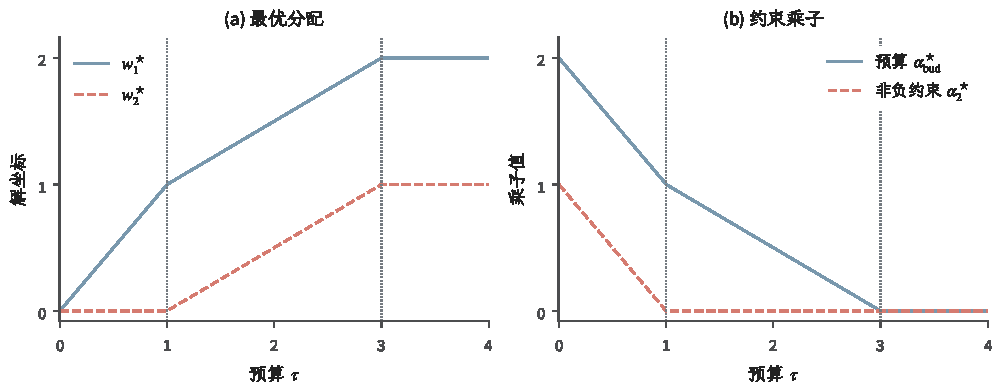
\includegraphics[width=\linewidth]{figures/math-preparation/concept-revision-analysis-functional/budget-active-set.pdf}
 \caption{例~\ref{ex:opt-kkt-budget}的解析解。左图为两个最优分配坐标，右图为预算乘子与第二个非负约束的乘子。竖参考线标出$\tau=1,3$；在切换点约束可以取等号而乘子为零，说明活跃性与正价格并不等价。}
 \label{fig:opt-budget-active-set}
\end{figure*}

一般地，设问题依赖参数$\tau$，活跃集在邻域内不变，把驻点条件、等式和活跃约束写成
$\bm{\Phi}(\bm{w},\bm{\nu},\bm{\alpha},\tau)=\bm{0}$。若对前三组变量的Jacobian
矩阵可逆，则第~\ref{chap:mathematical-analysis}章的隐式求导给出
\[
  \frac{d}{d\tau}
  \begin{bmatrix}\bm{w}^{\star}\\\bm{\nu}^{\star}\\\bm{\alpha}^{\star}\end{bmatrix}
  =
  -\left(\frac{\partial\bm{\Phi}}
  {\partial(\bm{w},\bm{\nu},\bm{\alpha})}\right)^{-1}
  \frac{\partial\bm{\Phi}}{\partial\tau}.
\]
这个Jacobian是完整KKT系统的导数，原目标Hessian可逆并不足以保证它可逆。活跃集改变或
该矩阵奇异时，解映射可能不可微；此时不能跨越切换点沿用同一个导数。

\subsection{原问题与对偶问题}
\label{sec:opt-duality}

\subsubsection{Lagrangian下界与弱对偶}

对固定乘子$\bm{\alpha}\geq\bm{0}$，任意可行$\bm{w}$都满足
$\mathcal{L}(\bm{w},\bm{\nu},\bm{\alpha})\leq f(\bm{w})$。因此
\term{对偶函数}（dual function）
\[
  q(\bm{\nu},\bm{\alpha})
  =\inf_{\bm{w}}\mathcal{L}(\bm{w},\bm{\nu},\bm{\alpha})
\]
给出原问题最优值的下界。最大化这个下界得到对偶问题。由构造立即有
$d^{\star}\leq p^{\star}$，称为\term{弱对偶}（weak duality）；差
$p^{\star}-d^{\star}$称为对偶间隙。对某组乘子取下确界得到$-\infty$，表示这组
乘子没有给出有限下界；对偶不可行则表示没有任何乘子满足对偶问题规定的可行条件。前者
描述一个候选乘子的函数值，后者描述整个候选集合，二者不能混用。

\subsubsection{Farkas择一与线性规划强对偶}

线性规划的强对偶可以从一个不可行证书推出。先建立所需的择一定理
\scite{math-boyd2004convex}

\begin{lemma}[有限生成锥的闭性]
\label{lem:opt-finitely-generated-cone}
给定$\bm{a}_1,\ldots,\bm{a}_r\in\mathbb{R}^m$，集合
\[
  K=\left\{\sum_{i=1}^r\alpha_i\bm{a}_i:\alpha_i\geq0\right\}
\]
是闭凸锥。
\end{lemma}

\begin{proof}
凸性和锥性质由非负线性组合直接得到。为证明闭性，先注意每个$\bm{x}\in K$都能由一组
线性无关的生成向量作非负组合。若某个表示使用的生成向量线性相关，就存在非零系数
$\bm{\gamma}$使$\sum_i\gamma_i\bm{a}_i=\bm{0}$；必要时改变符号，使至少一个
$\gamma_i>0$。从原系数中减去
$t\bm{\gamma}$，其中$t=\min_{\gamma_i>0}\alpha_i/\gamma_i$，仍保持所有系数
非负，并使至少一个系数变为零。重复此过程便得到线性无关的表示。

现取$\bm{x}^{(k)}\in K$且$\bm{x}^{(k)}\to\bm{x}$。线性无关的生成子集只有有限多个，
故可取子列，使每个$\bm{x}^{(k)}$都使用同一个子集$J$。以这些向量为列组成满列秩矩阵
$\bm{A}_J$，相应非负系数满足
\[
  \bm{\alpha}^{(k)}
  =(\bm{A}_J^{\top}\bm{A}_J)^{-1}\bm{A}_J^{\top}\bm{x}^{(k)}
  \longrightarrow
  (\bm{A}_J^{\top}\bm{A}_J)^{-1}\bm{A}_J^{\top}\bm{x}.
\]
极限系数仍逐项非负，且$\bm{x}$等于$\bm{A}_J$乘该极限系数，故$\bm{x}\in K$。
\end{proof}

\begin{lemma}[有限维多面体的线性像]
\label{lem:opt-polyhedral-image}
有限维多面体在线性映射下的像仍是多面体，因而是闭集。
\end{lemma}

\begin{proof}
设多面体$P=\{\bm{u}:\bm{B}\bm{u}\leq\bm{d}\}$，线性映射为
$\bm{v}=\bm{T}\bm{u}$。其图像
\[
  \{(\bm{u},\bm{v}):\bm{B}\bm{u}\leq\bm{d},\
  \bm{v}=\bm{T}\bm{u}\}
\]
是多面体，而$\bm{T}P$是该图像消去$\bm{u}$后的坐标投影。对一个待消变量，
Fourier--Motzkin消元分别收集其系数为正、为负和为零的不等式；每一对正、负系数
不等式消去该变量，零系数不等式原样保留。所得有限组非严格线性不等式恰好描述投影。
逐个消去$\bm{u}$的坐标，便得到$\bm{T}P$的有限线性不等式表示。多面体是有限个闭
半空间的交，因此闭。
\end{proof}

\begin{theorem}[Farkas择一定理]
\label{thm:opt-farkas}
给定$\bm{M}\in\mathbb{R}^{m\times d}$和$\bm{r}\in\mathbb{R}^m$，下列两个系统
恰有一个可行：
\[
  \bm{M}\bm{x}=\bm{r},\quad\bm{x}\geq\bm{0};
  \qquad
  \bm{M}^{\top}\bm{z}\geq\bm{0},\quad
  \bm{r}^{\top}\bm{z}<0.
\]
\end{theorem}

\begin{proof}
两者不能同时成立，因为若都成立，则
$0>\bm{r}^{\top}\bm{z}
=\bm{x}^{\top}\bm{M}^{\top}\bm{z}\geq0$，矛盾。
若第一个系统不可行，$\bm{r}$不属于锥
$K=\{\bm{M}\bm{x}:\bm{x}\geq\bm{0}\}$。它由$\bm{M}$的有限个列向量生成，故由
引理~\ref{lem:opt-finitely-generated-cone}可知$K$是闭凸锥。对$K$与$\bm{r}$应用
定理~\ref{thm:opt-projection-separation}，得到$\bm{a}$和$c$，使
$\langle\bm{a},\bm{k}\rangle\leq c<\langle\bm{a},\bm{r}\rangle$。
由于$\bm{0}\in K$，有$c\geq0$；又因为$t\bm{k}\in K$对所有$t\geq0$成立，
必有$\langle\bm{a},\bm{k}\rangle\leq0$，否则取充分大的$t$便会超过$c$。
令$\bm{z}=-\bm{a}$，可得$\langle\bm{z},\bm{r}\rangle<0$且
$\langle\bm{z},\bm{k}\rangle\geq0$对所有$\bm{k}\in K$成立。特别地，
对$\bm{M}$的每个列向量成立，故
$\bm{M}^{\top}\bm{z}\geq\bm{0}$。第二个系统可行。
\end{proof}

\begin{theorem}[有限维线性规划强对偶]
\label{thm:opt-lp-strong-duality}
考虑标准型原问题与对偶问题
\[
  \min_{\bm{x}\geq\bm{0}}\bm{c}^{\top}\bm{x}
  \quad\text{s.t.}\quad\bm{A}\bm{x}=\bm{b},
  \qquad
  \max_{\bm{y}}\bm{b}^{\top}\bm{y}
  \quad\text{s.t.}\quad\bm{A}^{\top}\bm{y}\leq\bm{c}.
\]
若原问题可行且有限下确界为$p^\star$，则原问题与对偶问题都有最优解，且两个最优值
都等于$p^\star$。
\end{theorem}

\begin{proof}
原始可行域
$P=\{\bm{x}:\bm{A}\bm{x}=\bm{b},\ \bm{x}\geq\bm{0}\}$是非空多面体。由
引理~\ref{lem:opt-polyhedral-image}，其目标值集合
\[
  W=\{\bm{c}^{\top}\bm{x}:\bm{x}\in P\}
\]
是$\mathbb{R}$中的非空多面体。集合$W$下有界，且一维多面体包含自己的有限下端点，
故$p^\star=\inf W$属于$W$。因此存在原始可行点$\bm{x}^{\star}$满足
$\bm{c}^{\top}\bm{x}^{\star}=p^\star$，原问题达到其最优值。

对任意$\varepsilon>0$，系统
\[
  \bm{A}\bm{x}=\bm{b},\quad
  \bm{c}^{\top}\bm{x}+s=p^\star-\varepsilon,\quad
  \bm{x}\geq\bm{0},\ s\geq0
\]
不可行，否则会有目标值小于$p^\star$的原始可行点。对增广矩阵应用
定理~\ref{thm:opt-farkas}，存在$(\bm{y}_{\varepsilon},\gamma_\varepsilon)$满足
\[
  \bm{A}^{\top}\bm{y}_{\varepsilon}
  +\gamma_\varepsilon\bm{c}\geq\bm{0},\quad
  \gamma_\varepsilon\geq0,\quad
  \bm{b}^{\top}\bm{y}_{\varepsilon}
  +\gamma_\varepsilon(p^\star-\varepsilon)<0.
\]
取任一原始可行$\bar{\bm{x}}$并与第一式作内积可知$\gamma_\varepsilon>0$，否则会与
最后一式矛盾。令
$\widehat{\bm{y}}_\varepsilon=-\bm{y}_\varepsilon/\gamma_\varepsilon$，便有
$\bm{A}^{\top}\widehat{\bm{y}}_\varepsilon\leq\bm{c}$且
$\bm{b}^{\top}\widehat{\bm{y}}_\varepsilon>p^\star-\varepsilon$。

记对偶可行多面体为
$D=\{\bm{y}:\bm{A}^{\top}\bm{y}\leq\bm{c}\}$。上面的构造说明$D$非空，且其
目标值集合
\[
  V=\{\bm{b}^{\top}\bm{y}:\bm{y}\in D\}
\]
对每个$\varepsilon>0$都包含一个大于$p^\star-\varepsilon$的值。弱对偶说明$V$中的
每个值都不超过$p^\star$，所以$\sup V=p^\star$。由
引理~\ref{lem:opt-polyhedral-image}，$V$是$\mathbb{R}$中的多面体；非空的一维
多面体只能是闭区间、闭射线、单点或整条实线。由于$V$有有限上确界，它必包含上端点
$p^\star$。因此存在$\bm{y}^{\star}\in D$使
$\bm{b}^{\top}\bm{y}^{\star}=p^\star$，对偶最优解达到与原问题相同的最优值。
\end{proof}

\begin{example}[二维资源分配的原始与对偶证书]
\label{ex:opt-resource-lp-duality}
考虑
\[
  \max_{x_1,x_2\geq0}3x_1+2x_2
  \quad\text{s.t.}\quad
  2x_1+x_2\leq4,\quad x_1+2x_2\leq4.
\]
为两类资源设置价格$u_1,u_2\geq0$。由于原问题是最大化，对可行点的资源余量按非负
价格计价会给出目标上界：
\begin{align*}
  \mathcal{L}(\bm{x},\bm{u})
  &=
  3x_1+2x_2
  +u_1(4-2x_1-x_2)+u_2(4-x_1-2x_2)\\
  &=
  4u_1+4u_2
  +(3-2u_1-u_2)x_1+(2-u_1-2u_2)x_2.
\end{align*}
要使$\sup_{\bm{x}\geq\bm{0}}\mathcal{L}(\bm{x},\bm{u})$有限，$x_1,x_2$的系数
必须非正，因而
$2u_1+u_2\geq3$且$u_1+2u_2\geq2$。此时上确界就是$4u_1+4u_2$，
最小化这个上界得到对偶
\[
  \min_{u_1,u_2\geq0}4u_1+4u_2
  \quad\text{s.t.}\quad
  2u_1+u_2\geq3,\quad u_1+2u_2\geq2.
\]
原始点$(x_1,x_2)=(4/3,4/3)$可行，值为$20/3$；对偶点
$(u_1,u_2)=(4/3,1/3)$可行，值也为$20/3$。弱对偶说明二者同时最优。两项资源约束
和两项产品约束均取等号，互补松弛也逐项成立。
\end{example}

\subsubsection{一般凸问题中的资格条件}

不可行、无界和未达到必须区分。Farkas向量证明约束不可行；若原问题沿可行射线无限改善，
弱对偶只说明不存在给出有限下界的对偶候选，也就是每个允许乘子的对偶函数值都为
$-\infty$，不能据此断言乘子候选集合为空。在线性规划标准型中，这种情形表现为对偶
不可行。若只有下确界而不达到，则不能展示原始最优点。一般凸问题在使用Slater条件前还需
处理低维定义域。沿用定义~\ref{def:opt-proper-domain-indicator}的有效定义域，还需说明低维集合中的“内部”。
\begin{definition}[仿射包与相对内部]
\label{def:opt-affine-hull-relative-interior}
对非空集合$C\subseteq\mathbb R^d$，其\term{仿射包}（affine hull）是全部有限仿射组合
$\sum_i\alpha_i\bm x_i$组成的集合，其中$\bm x_i\in C$、$\sum_i\alpha_i=1$，权重可为负。
点$\bm x\in C$属于\term{相对内部}（relative interior），是指存在$r>0$使
$B(\bm x,r)\cap\operatorname{aff}C\subseteq C$。
\end{definition}例如平面中的线段没有二维内部，但去掉两个端点后就是它的相对内部。

本章采用如下Slater版本。设$f$和不等式函数$g_k$都是适当凸函数，即它们不恒为
$+\infty$、从不取$-\infty$且至少在一点取有限值；这些函数具有共同凸定义域$D$，
等式约束为仿射约束$\bm{A}\bm{w}=\bm{b}$。若存在
\[
  \bar{\bm{w}}\in\operatorname{ri}D,\qquad
  \bm{A}\bar{\bm{w}}=\bm{b},\qquad
  g_k(\bar{\bm{w}})<0\quad\text{对所有 }k,
\]
并且原问题最优值有限，则原、对偶最优值相等，且存在最优对偶乘子。证明把可达到的
“约束余量—目标值”集合与严格低于原最优值的点分离；相对内部中的严格可行点排除了
目标系数为零的异常分离向量，归一化后便得到所需乘子。这里列出的定义域、仿射等式和
有限最优值都是所采用版本的一部分。凸性本身并不够，也不能把前面的线性规划证明原样
套到任意凸问题。第~\ref{chap:decision-theory-and-dynamic-risk}章会在状态、策略和
价值定义后，把同一对偶工具用于价值函数与占用度量。

\subsection{松弛与最优性证书}
\label{sec:opt-relaxations-certificates}

\subsubsection{凸包与可计算松弛}

第~\ref{chap:combinatorics}章已利用候选范围的包含关系建立松弛界。
现在还需区分两件事：连续集合能否精确包住原候选，以及返回的连续最优点能否恢复为原问题的解。
把原候选的加权平均一并纳入，可以得到包含这些候选的最小凸集。

\begin{definition}[有限点集的凸包]
\label{def:opt-convex-hull}
设$S=\{\bm s_1,\ldots,\bm s_N\}\subseteq\mathbb R^d$非空。
其凸包（convex hull）由这些点的全部凸组合构成：
\[
  \operatorname{conv}(S)
  =\left\{\sum_{i=1}^N\alpha_i\bm s_i:
  \alpha_i\geq0,\ \sum_{i=1}^N\alpha_i=1\right\}.
\]
\end{definition}
例如离散点集
\[
  S=\{(0,0),(1,0),(0,1)\}
\]
可以表示“至多选择一个项目”。把$S$替换为三角形
\[
  \operatorname{conv}(S)
  =\{(x_1,x_2):x_1,x_2\geq0,\ x_1+x_2\leq1\}
\]
得到\term{凸松弛}（convex relaxation）：原来的每个候选仍可行，但增加了分数候选。
对最小化问题，松弛最优值是原最优值的下界；对最大化问题则是上界。

对于有限非空$S$，精确凸包不改变任意线性目标$\bm{c}^{\top}\bm{x}$的最优值：任意
$\bm{x}=\sum_i\alpha_i\bm{s}_i\in\operatorname{conv}(S)$都满足
$\bm{c}^{\top}\bm{x}=\sum_i\alpha_i\bm{c}^{\top}\bm{s}_i
\geq\min_{\bm{s}\in S}\bm{c}^{\top}\bm{s}$，再结合
$S\subseteq\operatorname{conv}(S)$即得最小值相等，最大值同理。
数值相等仍没有指定求解器返回哪个点：若多个候选都最优，它们的凸组合也最优。

\begin{definition}[凸集的极点]
\label{def:opt-extreme-point}
设$K\subseteq\mathbb R^d$为凸集。若$\bm x\in K$满足：对任何$\bm u,\bm v\in K$
与$\theta\in(0,1)$，只要$\bm x=\theta\bm u+(1-\theta)\bm v$，就有
$\bm u=\bm v=\bm x$，则称$\bm x$为$K$的极点（extreme point）。
\end{definition}
极点不能再由其他可行点的非平凡平均得到。线性目标的所有最优点则组成同一个面。
\begin{definition}[线性目标的最优面]
\label{def:opt-optimal-face}
设线性目标$\bm c^\top\bm x$在非空凸集$K$上达到有限最大值$M$。
其最优面（optimal face）为
\[
  K^\star=\{\bm x\in K:\bm c^\top\bm x=M\}.
\]
最小化时，将$M$换为达到的有限最小值即可。
\end{definition}
当$K=\operatorname{conv}(S)$且$S$有限时，最优面正是$S$中全部最优点的凸包：
若一个凸组合对次优点给了正权重，其线性目标值便严格低于最大值。
若$S\subseteq\mathbb Z^d$，最优面还含有整数极点。可以在有限个整数最优点中，
按坐标次序逐项取最大值，选出一个点。若它是两个可行点的非平凡平均，线性最优性先迫使
这两个点都最优，再逐坐标的最大性迫使它们与所选点相同，因此该点确为极点。

即使如此，返回的最优点仍可能是分数点。例如上面的三角形在目标$x_1+x_2$下，
整条边$x_1+x_2=1$都是最优面，$(1/2,1/2)$也最优；逐坐标向上取整却得到
不属于原点集的$(1,1)$。整数极点的存在不保证任意分数最优点都能直接取整。

精确凸包的完整不等式描述可能难以获得。只保留局部约束通常
得到更大的多面体，计算较容易而界更松。也可以把乘积$x_ix_j$提升为矩阵变量并要求某个
块矩阵半正定，得到半正定松弛；它利用二次一致性，代价是矩阵锥约束更昂贵。

\subsubsection{上下界与最优性证书}

取整还可能破坏约束。考虑
\[
  \max_{x_1,x_2\in\{0,1\}}x_1+x_2
  \quad\text{s.t.}\quad 2x_1+2x_2\leq3.
\]
整数最优值为$1$，而把变量放宽到$[0,1]$后，$(3/4,3/4)$可行且目标值为$3/2$。
逐坐标四舍五入得到$(1,1)$，却违反容量约束；逐坐标向下取整虽可行，却得到目标值$0$。
因此松弛值、恢复可行性的规则和恢复后的目标损失必须分别分析。

若松弛集合比整数可行点的凸包更大，松弛最优值可能严格优于所有整数可行解；
这种最优值差异称为\term{整数间隙}（integrality gap）。上例采用加法差距时，间隙为
$3/2-1=1/2$。更大的松弛不一定产生严格间隙，它还取决于目标；
精确凸包对线性目标没有这种最优值差异，却仍可能包含分数最优点。

图~\ref{fig:opt-hull-relaxation}固定同一个整数问题，把两种连续可行域并列。
精确凸包上的最优值与整数候选一致；局部容量约束定义的松弛多出了整数候选无法平均
得到的区域。这一多出的区域，才使目标上界从$1$升到$3/2$。
\begin{figure*}[htbp]
 \centering
 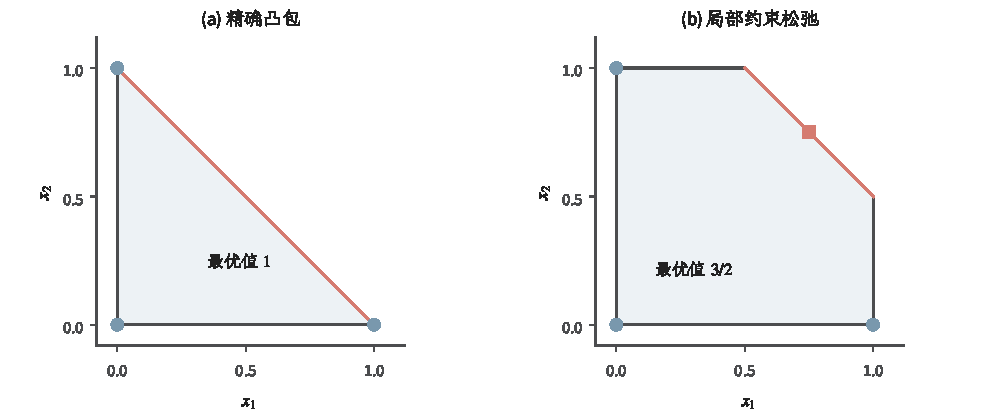
\includegraphics[width=\linewidth]{figures/math-preparation/concept-revision-analysis-functional/hull-relaxation.pdf}
 \caption{最大化$x_1+x_2$的两种放宽。左图精确凸包满足$x_1+x_2\leq1$；右图局部松弛满足$0\leq x_i\leq1$与$x_1+x_2\leq3/2$。实心圆为整数可行点，方形为右图的分数最优点$(3/4,3/4)$，粗边标出各自最优面。两图采用相同坐标尺度。}
 \label{fig:opt-hull-relaxation}
\end{figure*}

集合函数的连续扩展也有多种选择。连续变量上的凸性或凹性必须针对所选扩展检验，
不能仅凭原集合函数次模就断言成立；扩展方式决定可用的优化工具。
第~\ref{chap:graph-theory}章会讨论一个可精确求解的特殊情形：二值成对能量满足相应
次模不等式时，可以表示为非负容量的割。一般集合函数的次模性本身，并不保证任意
次模最大化或最小化都能用图割解决。

可计算界构成停止证书。对最小化问题，若可行解给出上界$U$，对偶或松弛给出下界$L$，
则
\[
  0\leq U-p^\star\leq U-L.
\]
当$U=L$时已证明全局最优。若把松弛解取整为可行解$\widehat{\bm{x}}$，还应单独分析
$f(\widehat{\bm{x}})-L$；“取整后看起来接近”不是误差界。互补松弛能够证明哪些约束在
最优点活跃，却不总能直接构造整数解。图模型中的边缘多面体和MAP松弛会在图与概率对象
建立后复用这里的凸包、上下界和间隙概念。

\section{光滑目标的迭代求解}
\label{sec:opt-smooth-iterative-methods}

有了可判定的最优性条件，还需构造能逐步接近它的参数序列。这里先限定目标可微且梯度光滑：
梯度下降用一阶信息保证单步改善，动量和预条件再利用迭代历史或曲率改变移动方向。
每种改进的保证都应与前节的曲率条件配对，而不能仅凭更新公式判断快慢。

\subsection{梯度下降与步长}
\label{sec:opt-gradient-descent}

\subsubsection{光滑上界与单步下降}

梯度给出最陡的一阶下降方向，但一步走多远取决于函数弯曲程度。光滑性把局部线性近似的
余项控制为二次量\scite{math-nocedal2006numerical}。本小节考虑可微函数
$f:\mathbb R^d\to\mathbb R$，并选取一个正的梯度Lipschitz上界$L>0$。
若梯度恒定，仍可选择任意正上界；这样后面的$1/L$步长也有定义。
全空间的设定保证更新点仍在函数定义域内；若目标只定义在开凸子域上，使用下降引理时
还须确认两端点及其线段留在该域内，不能直接把任意梯度步代入。

\begin{lemma}[下降引理]
\label{lem:opt-descent}
若$f:\mathbb R^d\to\mathbb R$可微且梯度是$L$-Lipschitz连续的，$L>0$，则对任意
$\bm u,\bm v\in\mathbb R^d$，
\begin{equation}
  f(\bm{v})\leq f(\bm{u})
  +\langle\nabla f(\bm{u}),\bm{v}-\bm{u}\rangle
  +\frac{L}{2}\lVert\bm{v}-\bm{u}\rVert_2^2.
  \label{eq:opt-descent-lemma}
\end{equation}
\end{lemma}

\begin{proof}
令$\bm{d}=\bm{v}-\bm{u}$。沿线段积分并减去一阶项可得
\[
  f(\bm{v})-f(\bm{u})-\langle\nabla f(\bm{u}),\bm{d}\rangle
  =
  \int_0^1
  \langle\nabla f(\bm{u}+t\bm{d})-\nabla f(\bm{u}),\bm{d}\rangle\,dt.
\]
由Cauchy--Schwarz不等式和梯度Lipschitz条件，被积函数至多为
$Lt\lVert\bm{d}\rVert_2^2$；积分即得结论。
\end{proof}

梯度下降按
\begin{equation}
  \bm{w}^{(t+1)}
  =\bm{w}^{(t)}-\eta\nabla f(\bm{w}^{(t)})
  \label{eq:opt-gradient-descent}
\end{equation}
更新。把$\bm{v}$取为右端点代入下降引理，得到
\begin{equation}
  f(\bm{w}^{(t+1)})
  \leq f(\bm{w}^{(t)})
  -\eta\left(1-\frac{L\eta}{2}\right)
  \lVert\nabla f(\bm{w}^{(t)})\rVert_2^2.
  \label{eq:opt-gradient-single-step}
\end{equation}
所以$0<\eta<2/L$保证每个非驻点处严格下降。若$f$下有界，记其有限下确界为
\[
  f_{\inf}:=\inf_{\bm{w}\in\mathbb{R}^d}f(\bm{w})>-\infty.
\]
取$\eta=1/L$并对$t=0,\ldots,T-1$求和，可得非凸光滑情形的保证
\begin{equation}
  \min_{0\leq t<T}\lVert\nabla f(\bm{w}^{(t)})\rVert_2^2
  \leq
  \frac{2L(f(\bm{w}^{(0)})-f_{\inf})}{T}.
  \label{eq:opt-nonconvex-gradient-rate}
\end{equation}
它只说明某次迭代接近驻点，没有声称驻点是全局最优点。

步长上界在一维二次函数上即可看到。对$f(w)=Lw^2/2$，
$w^{(t+1)}=(1-\eta L)w^{(t)}$。当$\eta=2/L$时迭代在正负之间等幅振荡；
$\eta>2/L$时幅度按$|1-\eta L|>1$增长。负梯度方向本身没有错，失败来自步长跨过了
曲率允许的稳定范围。

\subsubsection{不同曲率下的收敛证明}

若$f$还凸、最小点$\bm{w}^{\star}$存在，并继续取$\eta=1/L$，则由凸性有
$f(\bm{w}^{(t)})-f^\star
\leq\langle\nabla f(\bm{w}^{(t)}),\bm{w}^{(t)}-\bm{w}^{\star}\rangle$。
先展开距离平方并使用这个不等式：
\begin{align*}
  \lVert\bm{w}^{(t+1)}-\bm{w}^{\star}\rVert_2^2
  &=
  \lVert\bm{w}^{(t)}-\bm{w}^{\star}\rVert_2^2
  -\frac{2}{L}
  \left\langle\nabla f(\bm{w}^{(t)}),
  \bm{w}^{(t)}-\bm{w}^{\star}\right\rangle\\
  &\qquad
  +\frac{1}{L^2}\lVert\nabla f(\bm{w}^{(t)})\rVert_2^2\\
  &\leq
  \lVert\bm{w}^{(t)}-\bm{w}^{\star}\rVert_2^2
  -\frac{2}{L}\bigl(f(\bm{w}^{(t)})-f^\star\bigr)\\
  &\qquad
  +\frac{1}{L^2}\lVert\nabla f(\bm{w}^{(t)})\rVert_2^2.
\end{align*}
另一方面，把$\eta=1/L$代入式~\eqref{eq:opt-gradient-single-step}可得
\[
  \frac{1}{L^2}\lVert\nabla f(\bm{w}^{(t)})\rVert_2^2
  \leq
  \frac{2}{L}\bigl(
  f(\bm{w}^{(t)})-f(\bm{w}^{(t+1)})\bigr).
\]
用后一式消去梯度平方项，得到
\[
  \lVert\bm{w}^{(t+1)}-\bm{w}^{\star}\rVert_2^2
  \leq
  \lVert\bm{w}^{(t)}-\bm{w}^{\star}\rVert_2^2
  -\frac{2}{L}\bigl(f(\bm{w}^{(t+1)})-f^\star\bigr).
\]
对$t=0,\ldots,T-1$求和并去掉末端的非负距离，便有
\[
  \frac{2}{L}\sum_{t=0}^{T-1}
  \bigl(f(\bm{w}^{(t+1)})-f^\star\bigr)
  \leq
  \lVert\bm{w}^{(0)}-\bm{w}^{\star}\rVert_2^2.
\]
式~\eqref{eq:opt-gradient-single-step}还说明目标值单调不增，因此左侧求和中的每一项
都不小于$f(\bm{w}^{(T)})-f^\star$。于是
\begin{equation}
  f(\bm{w}^{(T)})-f^\star
  \leq\frac{L\lVert\bm{w}^{(0)}-\bm{w}^{\star}\rVert_2^2}{2T}.
  \label{eq:opt-convex-gradient-rate}
\end{equation}

若满足PL条件，把式~\eqref{eq:opt-pl-condition}代入
式~\eqref{eq:opt-gradient-single-step}，在$\eta=1/L$时得到
\begin{equation}
  f(\bm{w}^{(t)})-f^\star
  \leq
  \left(1-\frac{\mu}{L}\right)^t
  \bigl(f(\bm{w}^{(0)})-f^\star\bigr).
  \label{eq:opt-pl-linear-rate}
\end{equation}
强凸函数满足PL条件，还由
$f(\bm{w})-f^\star\geq\mu\lVert\bm{w}-\bm{w}^{\star}\rVert_2^2/2$
把目标误差转成参数误差。没有强凸时，式~\eqref{eq:opt-pl-linear-rate}不保证迭代趋向
某个唯一参数。

固定步长需要已知或估计$L$。回溯线搜索从候选步长开始缩小，直到
$f(\bm{w}-\eta\nabla f(\bm{w}))\leq
f(\bm{w})-c\eta\lVert\nabla f(\bm{w})\rVert_2^2$成立，其中$c\in(0,1)$。
学习率调度则预先或按进度改变$\eta_t$。线搜索用实际函数值核验当前一步，调度只规定时间
表；二者都不能弥补错误梯度或无下界目标。

\subsection{代理上界与单调改善}
\label{sec:opt-majorization-improvement}

梯度下降利用一个可计算二次上界。若上界来自别的可解结构，同一下降逻辑也能使用，
而不要求变量分块或目标本身是二次函数。
\begin{definition}[主化代理与MM更新]
\label{def:opt-majorization-minimization}
给定目标$F:C\to\mathbb R$、当前点$\bm w^{(t)}\in C$，
\term{主化--最小化方法}（majorization--minimization, MM）在当前点
$\bm{w}^{(t)}$构造代理函数$Q(\bm{w}\mid\bm{w}^{(t)})$，满足
\[
  F(\bm{w})\leq Q(\bm{w}\mid\bm{w}^{(t)}),
  \qquad
  F(\bm{w}^{(t)})=Q(\bm{w}^{(t)}\mid\bm{w}^{(t)}).
\]
上界关系要求对所有$\bm w\in C$成立。若新点$\bm w^{(t+1)}\in C$满足代理值不增，
就称这一步为MM改善更新。
\end{definition}
此时
\begin{align*}
  F(\bm{w}^{(t+1)})
  &\leq Q(\bm{w}^{(t+1)}\mid\bm{w}^{(t)})\\
  &\leq Q(\bm{w}^{(t)}\mid\bm{w}^{(t)})
  =F(\bm{w}^{(t)}).
\end{align*}
第一步用全局上界，第二步用代理改善，最后一步用切触条件。若代理只在当前点附近控制原
目标，而新点走出该邻域，单调链条便会断裂。

下降引理本身给出一个显式代理。若$F$为$L$光滑，可取
\[
  Q(\bm{w}\mid\bm{w}^{(t)})
  =F(\bm{w}^{(t)})
  +\langle\nabla F(\bm{w}^{(t)}),\bm{w}-\bm{w}^{(t)}\rangle
  +\frac{L}{2}\lVert\bm{w}-\bm{w}^{(t)}\rVert_2^2.
\]
它在当前点切触并全局上界$F$；精确最小化$Q$恰好得到步长$1/L$的梯度更新。仅让代理
与原目标在当前点具有相同梯度，却不满足全局上界，不能推出上面的单调不等式链。

例如$F(x)=x^2/2$、当前点$x^{(t)}=1$，取
$Q(x\mid1)=1/2+(x-1)+(x-1)^2$，则$Q-F=(x-1)^2/2\geq0$且当前点取等号。
代理最小点为$1/2$，于是$F(1/2)=1/8\leq Q(1/2\mid1)=1/4\leq F(1)=1/2$。
图~\ref{fig:opt-majorizer-versus-tangent}把这条链与只有相同局部斜率的切线对照。
\begin{figure}[htbp]
 \centering
 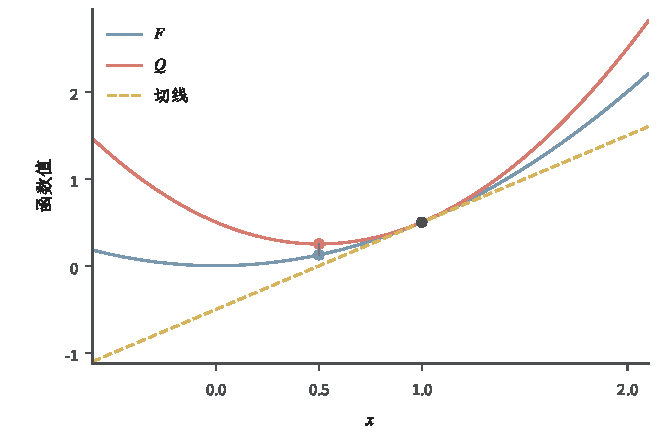
\includegraphics[width=\linewidth]{figures/math-preparation/reader-revision-analysis/optimization-majorizer-versus-tangent.pdf}
 \caption{代理上界与切线的区别。蓝线为$F(x)=x^2/2$，红线为当前点$1$处的主化代理$Q$，
 黄虚线为同点切线$x-1/2$。三者在当前点同值同斜率，但切线位于目标下方，
 最小化它不能使用MM的上界链；红点标出代理最小点对应的值。图为解析教学示例。}
 \label{fig:opt-majorizer-versus-tangent}
\end{figure}

\subsection{曲率、加速与预条件}
\label{sec:opt-curvature-acceleration}

梯度下降的收敛界已经显示，方向上的曲率差异会限制统一步长。
加速递推利用迭代历史，预条件则改变不同方向的尺度；牛顿法进一步用局部二阶近似。
这三种机制改变不同部分，条件与收益须分别对照，不能由一个二阶矩阵的出现就认定获得加速。

\subsubsection{动量与加速的递推结构}

对二次函数$f(\bm{w})=\frac12\bm{w}^{\top}\bm{H}\bm{w}
-\bm{c}^{\top}\bm{w}$，梯度下降的误差满足
$\bm{e}^{(t+1)}=(\bm{I}-\eta\bm{H})\bm{e}^{(t)}$。当
$\bm{H}\succ\bm{0}$但条件数$\kappa=L/\mu$很大时，同一步长必须同时照顾陡峭与平坦
方向，平坦方向因而收敛缓慢。

\term{动量法}（momentum method）保存过去方向：
\[
  \bm{v}^{(t+1)}=\beta\bm{v}^{(t)}+\nabla f(\bm{w}^{(t)}),
  \qquad
  \bm{w}^{(t+1)}=\bm{w}^{(t)}-\eta\bm{v}^{(t+1)}.
\]
它通过二阶递推重塑各特征方向上的多项式响应，但$\beta$和$\eta$不能各自独立地任取。
对上述正定二次目标，曲率为$\lambda_i$的特征方向满足
\[
  e_i^{(t+1)}
  =(1+\beta-\eta\lambda_i)e_i^{(t)}-\beta e_i^{(t-1)}.
\]
该方向的两个特征根都严格位于单位圆内，当且仅当
$-1<\beta<1$且$0<\eta\lambda_i<2(1+\beta)$。因而常用的
$0\leq\beta<1$还须配合$0<\eta<2(1+\beta)/L$，才能保证所有方向稳定。
若已知$0<\mu\leq\lambda_i\leq L$，经典重球参数
\[
  \eta=\frac{4}{(\sqrt{L}+\sqrt{\mu})^2},
  \qquad
  \beta=\left(\frac{\sqrt{L}-\sqrt{\mu}}
  {\sqrt{L}+\sqrt{\mu}}\right)^2
\]
给出这一二次模型上的代表性最坏方向速率；它不是一般非凸目标或含噪梯度下的无条件
调参规则。

\term{Nesterov加速梯度}
（Nesterov accelerated gradient）在前瞻点计算梯度：
\[
  \bm{z}^{(t)}=\bm{w}^{(t)}+\beta_t(\bm{w}^{(t)}-\bm{w}^{(t-1)}),
  \qquad
  \bm{w}^{(t+1)}=\bm{z}^{(t)}-\frac1L\nabla f(\bm{z}^{(t)}).
\]
令$\bm{w}^{(-1)}=\bm{w}^{(0)}$、$q_0=1$，并取
\[
  q_{t+1}=\frac{1+\sqrt{1+4q_t^2}}{2},
  \qquad
  \beta_t=\frac{q_t-1}{q_{t+1}}.
\]
若$f$为凸可微函数、梯度$L$-Lipschitz连续、最小点存在，并且每步使用精确梯度和
步长$1/L$，则上述选择给出
$f(\bm{w}^{(t)})-f^\star=O(1/t^2)$；同样条件下，普通梯度下降的一般保证为
$O(1/t)$。强凸时还可采用依赖$\mu/L$的固定系数得到线性速率，但那是另一组参数和证明。
在一维二次函数$f(w)=\lambda w^2/2$上，这个迭代可直接核验为
\[
  w^{(t+1)}
  =\left(1-\frac{\lambda}{L}\right)
  \bigl((1+\beta_t)w^{(t)}-\beta_t w^{(t-1)}\bigr).
\]
当$\lambda=L$时一步到达零点；当$\lambda\ll L$时，跨步项改变平坦方向上的二阶递推，
但系数选错仍会振荡。一般凸证明不能只检查这个二次算例，而是构造同时含目标误差与外推
距离的势函数；$q_{t+1}^2-q_{t+1}=q_t^2$使相邻两步的耦合项抵消，最终留下
$q_t^2(f(\bm{w}^{(t)})-f^\star)$的统一上界。加速结论因此来自特定外推序列与势函数
不等式，不能由“加入惯性”本身推出。

\subsubsection{牛顿法、近似曲率与预条件}

\term{牛顿法}（Newton's method）在$\bm{w}^{(t)}$处使用关于增量$\bm{p}$的局部
二次模型
\[
  m_t(\bm{p})
  =
  f(\bm{w}^{(t)})
  +\left\langle\nabla f(\bm{w}^{(t)}),\bm{p}\right\rangle
  +\frac12\bm{p}^{\top}\nabla^2f(\bm{w}^{(t)})\bm{p}.
\]
令$\nabla_{\bm{p}}m_t(\bm{p}^{(t)})=\bm{0}$，便得到牛顿方程
\[
  \nabla^2 f(\bm{w}^{(t)})\bm{p}^{(t)}
  =-\nabla f(\bm{w}^{(t)}),\qquad
  \bm{w}^{(t+1)}=\bm{w}^{(t)}+\alpha_t\bm{p}^{(t)}.
\]
若Hessian矩阵在最优点附近正定且Lipschitz连续，取单位步长可得到局部二次收敛。但Hessian矩阵
不定时，牛顿方向未必下降；离最优点较远时还需线搜索或信赖域。

对非线性最小二乘
$f(\bm{w})=\frac12\lVert\bm{r}(\bm{w})\rVert_2^2$，设
$\bm{r}:\mathbb{R}^d\to\mathbb{R}^m$。记残差向量的Jacobian矩阵为
$\bm{J}(\bm{w})\in\mathbb{R}^{m\times d}$，其第$i$行为
$\bm{J}_{i,:}(\bm{w})=\nabla r_i(\bm{w})^{\top}$，则
\[
  \nabla^2f(\bm{w})
  =\bm{J}(\bm{w})^{\top}\bm{J}(\bm{w})
  +\sum_{i=1}^m r_i(\bm{w})\nabla^2r_i(\bm{w}).
\]
\term{Gauss--Newton法}忽略第二项，使用半正定矩阵
$\bm{J}^{\top}\bm{J}$。当残差小或残差函数近似线性时近似合理；残差大时，省略项可能
决定曲率。

\term{拟牛顿法}（quasi-Newton method）不显式计算Hessian矩阵，而用梯度差
$\bm{y}^{(t)}=\nabla f(\bm{w}^{(t+1)})-\nabla f(\bm{w}^{(t)})$和步长
$\bm{s}^{(t)}=\bm{w}^{(t+1)}-\bm{w}^{(t)}$更新矩阵近似，并满足割线条件
$\bm{B}^{(t+1)}\bm{s}^{(t)}=\bm{y}^{(t)}$。若$\bm{B}^{(t)}$近似Hessian矩阵，
BFGS更新为
\begin{equation}
  \bm{B}^{(t+1)}
  =
  \bm{B}^{(t)}
  +
  \frac{\bm{y}^{(t)}(\bm{y}^{(t)})^{\top}}
       {(\bm{y}^{(t)})^{\top}\bm{s}^{(t)}}
  -
  \frac{\bm{B}^{(t)}\bm{s}^{(t)}(\bm{s}^{(t)})^{\top}\bm{B}^{(t)}}
       {(\bm{s}^{(t)})^{\top}\bm{B}^{(t)}\bm{s}^{(t)}}.
  \label{eq:opt-bfgs-update}
\end{equation}
当$\bm{B}^{(t)}\succ\bm{0}$且曲率条件
$(\bm{y}^{(t)})^{\top}\bm{s}^{(t)}>0$成立时，
式~\eqref{eq:opt-bfgs-update}保持$\bm{B}^{(t+1)}\succ\bm{0}$，相应搜索方向
$-(\bm{B}^{(t+1)})^{-1}\nabla f$才由正定性保证是下降方向。沿下降方向执行满足
Wolfe条件的线搜索可产生该正曲率内积。具体地，令
$\bm{w}^{(t+1)}=\bm{w}^{(t)}+\alpha_t\bm{p}^{(t)}$，其中
$\nabla f(\bm{w}^{(t)})^{\top}\bm{p}^{(t)}<0$。Wolfe条件要求存在
$0<c_1<c_2<1$使
\begin{equation}
\begin{aligned}
  f(\bm{w}^{(t+1)})
  &\leq
  f(\bm{w}^{(t)})
  +
  c_1\alpha_t
  \nabla f(\bm{w}^{(t)})^{\top}\bm{p}^{(t)},\\
  \nabla f(\bm{w}^{(t+1)})^{\top}\bm{p}^{(t)}
  &\geq
  c_2\nabla f(\bm{w}^{(t)})^{\top}\bm{p}^{(t)}.
\end{aligned}
\label{eq:opt-wolfe-conditions}
\end{equation}
第二行就是\term{Wolfe曲率条件}（Wolfe curvature condition）。由
$\bm{s}^{(t)}=\alpha_t\bm{p}^{(t)}$可得
\[
  (\bm{y}^{(t)})^{\top}\bm{s}^{(t)}
  \geq
  \alpha_t(c_2-1)
  \nabla f(\bm{w}^{(t)})^{\top}\bm{p}^{(t)}
  >0.
\]
非凸或梯度含噪时，上述条件可能难以满足，此时可能需要阻尼或跳过更新。

\term{预条件}（preconditioning）则选择正定矩阵$\bm{P}$，按
\[
  \bm{w}^{(t+1)}
  =
  \bm{w}^{(t)}-\eta\bm{P}\nabla f(\bm{w}^{(t)})
\]
更新。
这等价于在新的坐标或内积下做最陡下降。若\(p_i>0\)，并且
\[
  \bm{P}
  =
  \bm{Q}\operatorname{diag}(p_1,\ldots,p_d)\bm{Q}^{\top},
\]
则定义
\[
  \bm{P}^{1/2}
  =
  \bm{Q}\operatorname{diag}(\sqrt{p_1},\ldots,\sqrt{p_d})\bm{Q}^{\top}.
\]
这就是$\bm{P}$唯一的对称正定平方根：它满足
$\bm{P}^{1/2}\bm{P}^{1/2}=\bm{P}$，并且可逆，其逆记为$\bm{P}^{-1/2}$。
对当前正定二次目标，记
\[
  \widetilde{\bm{H}}=\bm{P}^{1/2}\bm{H}\bm{P}^{1/2},
  \qquad
  0<\widetilde{\mu}
  =\lambda_{\min}(\widetilde{\bm{H}})
  \leq\lambda_{\max}(\widetilde{\bm{H}})
  =\widetilde{L}.
\]
原坐标中的误差递推为
$\bm{e}^{(t+1)}=(\bm{I}-\eta\bm{P}\bm{H})\bm{e}^{(t)}$。令
$\widetilde{\bm{e}}^{(t)}=\bm{P}^{-1/2}\bm{e}^{(t)}$，则
\[
  \widetilde{\bm{e}}^{(t+1)}
  =
  (\bm{I}-\eta\widetilde{\bm{H}})
  \widetilde{\bm{e}}^{(t)},
  \qquad
  \bm{P}^{-1/2}
  (\bm{I}-\eta\bm{P}\bm{H})
  \bm{P}^{1/2}
  =
  \bm{I}-\eta\widetilde{\bm{H}}.
\]
右侧矩阵由可逆坐标变换$\bm{P}^{1/2}$得到，因而与原误差递推矩阵相似；相似矩阵具有
相同特征值。由于$\widetilde{\bm{H}}$对称正定，迭代对任意初始误差收敛当且仅当
$0<\eta<2/\widetilde{L}$。取
$\eta=2/(\widetilde{L}+\widetilde{\mu})$时，在变换后的欧氏范数中，每步最坏收缩因子为
\[
  \frac{\widetilde{\kappa}-1}{\widetilde{\kappa}+1},
  \qquad
  \widetilde{\kappa}
  =\frac{\widetilde{L}}{\widetilde{\mu}}.
\]
因此预条件的目标不是单独让$\bm{P}$的条件数小，而是让变换后曲率
$\widetilde{\bm{H}}$的条件数接近$1$。固定$\bm{P}\succ\bm{0}$只保证定义了合法内积；
若它与$\bm{H}$不匹配，$\widetilde{\kappa}$反而可能增大。对一般二阶可微的光滑强凸
函数，需要在所有迭代经过的区域统一满足
$\widetilde{\mu}\bm{I}\preceq
\bm{P}^{1/2}\nabla^2f(\bm{w})\bm{P}^{1/2}
\preceq\widetilde{L}\bm{I}$，上述步长范围与线性收敛解释才相应延续；变化的预条件矩阵还需
额外控制。

动量利用历史更新，牛顿类近似当前曲率，预条件改变几何尺度；三者可能组合，却不是同一种
机制。第~\ref{chap:matrix-analysis}章将在矩阵函数与Kronecker结构建立后给出结构化
预条件，Fisher矩阵与经验梯度二阶矩的差别则需等概率对象建立后讨论。

\begin{example}[两个曲率方向上的预条件]
\label{ex:opt-anisotropic-preconditioning}
取$f(\bm w)=(w_1^2+16w_2^2)/2$，初值$(2,2)^{\top}$。普通梯度下降若取
$\eta=0.1$，两个坐标分别乘以$0.9$与$-0.6$，因而
$\bm w^{(t)}=(2\times0.9^t,\,2\times(-0.6)^t)^{\top}$。
第二坐标来回越过谷底，第一坐标却缓慢缩小。取
$\bm P=\operatorname{diag}(1,1/16)$及$\eta=1/2$后，
$\bm P\nabla f(\bm w)=\bm w$，两坐标每步都减半。
\end{example}

\begin{figure*}[htbp]
 \centering
 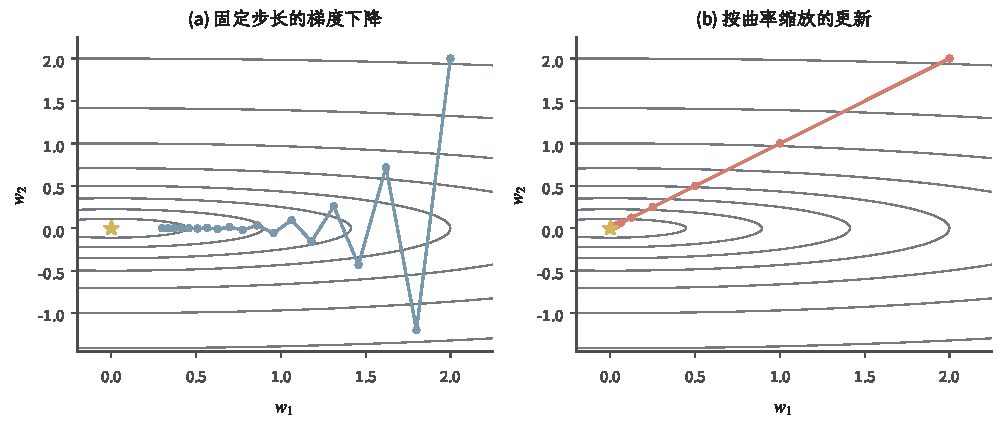
\includegraphics[width=\linewidth]{figures/math-preparation/analysis-geometry/optimization-preconditioned-paths.pdf}
 \caption{例~\ref{ex:opt-anisotropic-preconditioning}中的精确更新路径。灰线是同一二次目标的等值线，蓝、红圆点分别表示普通更新与预条件更新，黄色星号是最小点。预条件使用了已知曲率，获得和应用这一矩阵的成本仍属于算法代价。}
 \label{fig:opt-preconditioned-paths}
\end{figure*}

这个例子中的预条件恰好消除了两个方向的尺度差。一般目标的曲率会随位置变化，近似矩阵
也有误差；因此图中的直达路径解释机制，不构成所有预条件方法都更快的保证。

\section{非光滑与随机目标的求解}
\label{sec:opt-nonsmooth-stochastic-methods}

接下来改变的是算法能取得的局部信息。绝对值等正则项使普通梯度不存在，
大规模数据又可能只允许计算带噪声的梯度估计。非光滑性和随机性是两种不同障碍：
前者需要次梯度或邻近映射，后者需要控制误差积累；两者可以出现在同一个问题中。

\subsection{非光滑目标与正则化}
\label{sec:opt-nonsmooth-proximal}

\subsubsection{次梯度与非光滑最优性}

绝对值损失和$\ell_1$稀疏惩罚在零点不可微，但凸函数仍可用支撑直线描述。
\begin{definition}[凸次梯度与次微分]
\label{def:opt-convex-subgradient}
设$f:\mathbb R^d\to\mathbb R\cup\{+\infty\}$为适当凸函数，$f(\bm u)$有限。
向量$\bm{g}\in\mathbb R^d$若满足
\[
  f(\bm{v})\geq f(\bm{u})+\langle\bm{g},\bm{v}-\bm{u}\rangle
  \quad\text{对所有 }\bm{v},
\]
就称为$f$在$\bm{u}$处的\term{次梯度}（subgradient）。全部次梯度组成
$\partial f(\bm{u})$，称为次微分；它可以是空集。
\end{definition}
例如
\[
  \partial |x|=
  \begin{cases}
    \{1\},&x>0,\\
    [-1,1],&x=0,\\
    \{-1\},&x<0.
  \end{cases}
\]
凸函数在$\bm{w}^{\star}$处最优，当且仅当
$\bm{0}\in\partial f(\bm{w}^{\star})$。若零向量是次梯度，定义立即给出
$f(\bm{v})\geq f(\bm{w}^{\star})$；反过来，若$\bm{w}^{\star}$全局最优，则
$f(\bm{v})\geq f(\bm{w}^{\star})+\langle\bm{0},\bm{v}-\bm{w}^{\star}\rangle$，
所以零向量满足次梯度定义。这个等价性依赖凸次梯度采用全局下界定义。
若要把$f+r$的次微分直接写成$\partial f+\partial r$，或把约束写成指标函数后拆分
次微分，还需共同相对内部等相应资格条件；不能只凭两个函数都凸就无条件使用求和等式。

\subsubsection{投影、邻近与软阈值}

对闭凸集$C$，欧氏\term{投影}（projection）
$\Pi_C(\bm{z})=\argmin_{\bm{w}\in C}\lVert\bm{w}-\bm{z}\rVert_2^2$
把一步梯度更新拉回可行域：
\[
  \bm{w}^{(t+1)}
  =\Pi_C\bigl(\bm{w}^{(t)}-\eta_t\nabla f(\bm{w}^{(t)})\bigr).
\]
定理~\ref{thm:opt-projection-separation}的证明已经说明，在有限维空间中，非空闭性保证
最近点存在，而凸性与平方距离的严格凸性共同保证唯一。若$C$非凸，最近点可能不唯一。

投影处理一个硬可行域；若希望保留整个空间中的候选，却对不同候选收取不同惩罚，
就要在“惩罚小”和“离当前点近”之间取得平衡。
\begin{definition}[凸函数的邻近算子]
\label{def:opt-proximal-operator}
设$r:\mathbb R^d\to\mathbb R\cup\{+\infty\}$适当、下半连续且凸，$\eta>0$。
函数$r$的\term{邻近算子}（proximal operator）定义为
\[
  \operatorname{prox}_{\eta r}(\bm{z})
  =\argmin_{\bm{w}}
  \left\{r(\bm{w})+\frac{1}{2\eta}
  \lVert\bm{w}-\bm{z}\rVert_2^2\right\}.
\]
\end{definition}
这里的$\eta$调节惩罚与距离的相对权重；它还未指代某个算法的迭代步数。二次项使目标强凸。
适当闭凸函数具有仿射下界，二次项在无穷远处超过这个下界的线性下降，所以子问题强制；
强制性与下半连续性保证最小点存在，强凸性保证它唯一，所以邻近算子对每个$\bm{z}$都有
单值输出。
指标函数$\iota_C$在$C$上为零、在外部为$+\infty$，其邻近算子正是投影。
对$f+r$，近端梯度先按光滑部分$f$走一步，再用$r$的邻近算子处理非光滑结构。

\begin{theorem}[$\ell_1$邻近算子是软阈值]
\label{thm:opt-soft-threshold}
设$\lambda\geq0$、$\eta>0$。对$r(\bm{w})=\lambda\lVert\bm{w}\rVert_1$，
\[
  [\operatorname{prox}_{\eta r}(\bm{z})]_j
  =\operatorname{sign}(z_j)\max\{|z_j|-\eta\lambda,0\}.
\]
\end{theorem}

\begin{proof}
目标按坐标可分，只需最小化
$\lambda|w|+(w-z)^2/(2\eta)$。若$w>0$，驻点为
$w=z-\eta\lambda$，只在$z>\eta\lambda$时落在该区域；若$w<0$，驻点为
$w=z+\eta\lambda$，只在$z<-\eta\lambda$时有效。若
$|z|\leq\eta\lambda$，零点最优性条件
$0\in\lambda[-1,1]-z/\eta$成立，所以$w=0$。合并三种情形即得结论。
\end{proof}

例如取$\bm z=(3,0.4,-2)^{\top}$与$\eta\lambda=1$，软阈值输出
$(2,0,-1)^{\top}$；小幅坐标被直接置零。若改用
$r(\bm w)=\lambda\lVert\bm w\rVert_2^2/2$，逐坐标驻点给出
$\operatorname{prox}_{\eta r}(\bm z)=\bm z/(1+\eta\lambda)$，在同一参数下为
$(1.5,0.2,-1)^{\top}$。两种正则化都缩小幅度，只有前者在这个例子中产生精确零值。

图~\ref{fig:opt-proximal-comparison}对同一个标量输入$z$比较三种处理：区间投影把
超出范围的值截到边界；软阈值把小幅值置零、其余幅值减去固定量；二次惩罚则等比例
缩小所有输入。投影保持可行性，软阈值产生稀疏性，二次惩罚改变幅度，它们都可以写成
邻近算子，但输出行为和所解决的问题不同。
\begin{figure}[htbp]
 \centering
 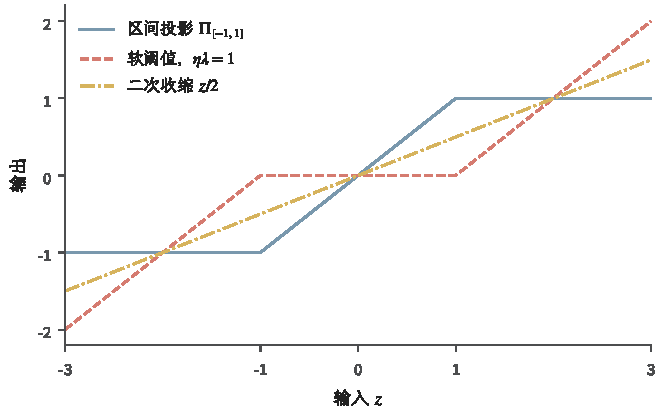
\includegraphics[width=\linewidth]{figures/math-preparation/concept-revision-analysis-functional/proximal-comparison.pdf}
 \caption{同一输入$z$的三种邻近映射。投影采用$C=[-1,1]$；软阈值与二次收缩均取$\eta\lambda=1$，分别输出$\operatorname{sign}(z)(|z|-1)_+$和$z/2$。横轴刻度标出阈值位置，曲线由完整分段解析式生成。}
 \label{fig:opt-proximal-comparison}
\end{figure}

邻近算子不会放大输入距离。令
$\bm{p}=\operatorname{prox}_{\eta r}(\bm{x})$、
$\bm{q}=\operatorname{prox}_{\eta r}(\bm{y})$。最优性条件给出
$(\bm{x}-\bm{p})/\eta\in\partial r(\bm{p})$和
$(\bm{y}-\bm{q})/\eta\in\partial r(\bm{q})$。把两个次梯度不等式相加，得到
\[
  \langle\bm{x}-\bm{y},\bm{p}-\bm{q}\rangle
  \geq\lVert\bm{p}-\bm{q}\rVert_2^2.
\]
再用Cauchy--Schwarz不等式便有
$\lVert\bm{p}-\bm{q}\rVert_2\leq\lVert\bm{x}-\bm{y}\rVert_2$。
这个非扩张性质依赖凸次梯度的单调性；非凸邻近子问题可能多解，不能直接沿用。

本节的凸次梯度也不同于第~\ref{chap:mathematical-analysis}章介绍的Clarke广义梯度。
前者用一个全局仿射下界定义，直接产生凸最优性条件；后者取局部Lipschitz函数邻近可微点
梯度极限的闭凸包，允许非凸局部结构。人为指定的替代梯度更只是反向计算信号，未必属于
前面任一集合。三者名称相近，定义对象与可用结论并不相同。

\begin{table*}[htbp]
 \centering\small
 \begin{tabularx}{\linewidth}{@{}lXX@{}}
 \toprule
 更新方式 & 每步处理的结构 & 分析前需核对的条件\\
 \midrule
 梯度下降 & 使用可微目标的梯度 & 光滑常数与步长；全局最优保证还依赖凸性或PL等条件\\
 投影梯度 & 梯度更新后求可行集最近点 & 非空闭凸集；投影本身的计算成本\\
 次梯度更新 & 使用非光滑凸目标的全局下界斜率 & 次梯度范数及步长序列；单步目标未必下降\\
 近端梯度 & 光滑部分求梯度，非光滑部分求邻近解 & 光滑部分的步长、正则项的适当闭凸性及可解邻近子问题\\
 \bottomrule
 \end{tabularx}
 \caption{常见一阶更新的结构与条件。相近的更新形式并不共享同一收敛定理。}
 \label{tab:opt-first-order-structures}
\end{table*}

\subsubsection{惩罚、约束与参数表达}

惩罚与硬约束有联系，但不是逐参数自动等价。考虑约束问题
\[
  \min_{\bm{w}}f(\bm{w})
  \quad\text{s.t.}\quad
  \lVert\bm{w}\rVert_1\leq R.
\]
若该问题有原始最优解，强对偶成立，并且对偶最优乘子
$\lambda^\star$确实达到，例如满足前述Slater条件且最优值有限，则原始最优解同时最小化
$f(\bm{w})+\lambda^\star\lVert\bm{w}\rVert_1$；Lagrangian中的常数
$-\lambda^\star R$不影响最小点。仅有原、对偶最优值相等并不能保证这样的有限乘子存在。
反过来，不同$\lambda$对应的范数半径可能相同，非凸问题还可能存在对偶间隙。把
$\bm{w}$写成其他参数的函数也会改变优化几何；即使表示同一预测函数，也不保证产生同一
更新轨迹。

同样的区别出现在权重衰减中。普通欧氏梯度下降用于
$f(\bm{w})+\lambda\lVert\bm{w}\rVert_2^2/2$时给出
\[
  \bm{w}^{(t+1)}
  =(1-\eta\lambda)\bm{w}^{(t)}-\eta\nabla f(\bm{w}^{(t)}),
\]
与直接乘上衰减因子相同。若使用预条件矩阵$\bm{P}$，惩罚梯度产生
$-\eta\lambda\bm{P}\bm{w}^{(t)}$，而坐标无关的直接衰减仍为
$-\eta\lambda\bm{w}^{(t)}$；除非$\bm{P}=\bm{I}$或另有匹配，它们不再相同。

\subsection{随机梯度与更新稳定性}
\label{sec:opt-stochastic-gradient-stability}

\subsubsection{随机梯度与带误差迭代}

有限和目标
\[
  F_S(\bm{w})=\frac1n\sum_{i=1}^n\ell_i(\bm{w})
  +\frac{\lambda}{2}\lVert\bm{w}\rVert_2^2
\]
的经验损失梯度要读取全部$n$项。这里的抽取先只用有限概率权重理解，$\mathbb E_I$表示按这些权重求和；
条件期望和随机收敛留待概率与随机过程章节。若$I$在$\{1,\ldots,n\}$上均匀抽取，则完整目标的
随机梯度可取
\[
  \bm{g}_I(\bm{w})
  =\nabla\ell_I(\bm{w})+\lambda\bm{w},\qquad
  \mathbb{E}_I[\bm{g}_I(\bm{w})]
  =\nabla F_S(\bm{w}).
\]
若按概率$p_i>0$非均匀抽取，则应改用
\[
  \bm{g}_I(\bm{w})
  =\frac{\nabla\ell_I(\bm{w})}{np_I}+\lambda\bm{w}.
\]
正则项梯度$\lambda\bm{w}$是确定量，无需抽样；小批量只需平均若干经过相应加权的
损失梯度，再加上这项确定梯度。小批量降低方差，却增加每步计算。

在概率工具建立前，可以先分析带确定误差的更新
\[
  \bm{w}^{(t+1)}
  =\bm{w}^{(t)}-\eta_t
  \bigl(\nabla F(\bm{w}^{(t)})+\bm{e}^{(t)}\bigr).
\]
若$F$为$L$光滑且$0<\eta_t\leq1/L$，把这一步代入下降引理，并对交叉项使用
Cauchy--Schwarz与$2ab\leq a^2+b^2$，可得
\[
  F(\bm{w}^{(t+1)})
  \leq F(\bm{w}^{(t)})
  -\frac{\eta_t}{2}\lVert\nabla F(\bm{w}^{(t)})\rVert_2^2
  +\frac{\eta_t}{2}\lVert\bm{e}^{(t)}\rVert_2^2.
\]
误差项因而必须与所求结论一起累计。固定非零偏差通常只允许迭代接近一个误差邻域；
$\sum_t\eta_t\lVert\bm{e}^{(t)}\rVert_2^2<\infty$使上述目标下降不等式中的累计
误差项有限。仅令
$\eta_t\to0$仍不够，还要核对步长总量是否足以持续纠偏，以及目标与迭代是否保持稳定。

若理想更新映射$T_t(\bm{w})=\bm{w}-\eta_t\nabla F(\bm{w})$是
$\rho_t$-Lipschitz，实际轨迹与理想轨迹之差$\delta_t$满足
\begin{equation}
  \delta_{t+1}\leq\rho_t\delta_t+\eta_t\lVert\bm{e}^{(t)}\rVert_2.
  \label{eq:opt-inexact-gradient-recurrence}
\end{equation}
展开递推可见，$\rho_t<1$时旧误差会衰减；若只有$\rho_t\leq1$，直接求和控制轨迹偏差
需要考察$\sum_t\eta_t\lVert\bm{e}^{(t)}\rVert_2$，前面的平方误差条件一般不能推出
这个一次范数条件。若$\rho_t>1$，传播因子还可能放大早期扰动。减小步长降低单步误差
影响，也会减慢理想更新。

\subsubsection{成对迭代与梯度自界}

同一递推可比较只替换一个样本的数据集$S,S'$。若每个样本梯度有界，且两条轨迹在使用
相同样本时由收缩映射拉近，只在抽到被替换样本时受到额外扰动，就能控制
$\lVert\bm{w}_S^{(t)}-\bm{w}_{S'}^{(t)}\rVert_2$。具体地，设每个样本梯度
$L$-Lipschitz且范数不超过$G$，两条迭代使用相同索引$I_t$。记距离为$\Delta_t$；
若$I_t$不是被替换的索引，则
\[
  \Delta_{t+1}\leq(1+\eta_tL)\Delta_t;
\]
若恰好抽到被替换项，则再增加至多$2\eta_tG$。在凸光滑且步长适当时，共同样本的梯度
更新可进一步证明为非扩张映射，从而去掉前式中的膨胀因子。这称为
\term{算法稳定性}（algorithmic stability）：训练集改动一个样本时，输出不会变化太大。
完整的期望界和随机收敛需使用第~\ref{chap:stochastic-processes-and-approximation}章的
条件期望与噪声工具。

缩放损失会等比例缩放梯度，因此学习率不能脱离损失尺度比较。梯度裁剪把过大更新限制在
指定半径内，改变了估计量并可能引入偏差。对更新式直接减去
$\eta\lambda\bm{w}$的权重衰减，在普通梯度下降中等价于$\ell_2$惩罚；使用坐标自适应缩放
时，两者通常不再等价。

\begin{lemma}[非负光滑函数的梯度自界]
\label{lem:opt-self-bounding}
若$\ell:\mathbb{R}^d\to[0,\infty)$可微且$L$光滑，其中$L>0$，则
\[
  \lVert\nabla\ell(\bm{w})\rVert_2^2\leq2L\ell(\bm{w}).
\]
\end{lemma}

\begin{proof}
在下降引理中取
$\bm{v}=\bm{w}-\nabla\ell(\bm{w})/L$，得到
\[
  \ell(\bm{v})
  \leq\ell(\bm{w})-\frac{1}{2L}
  \lVert\nabla\ell(\bm{w})\rVert_2^2.
\]
左侧非负，移项即得结论。若损失可取负值，这一步失效；给函数加常数虽不改变梯度，却会
改变右侧，所以非负性是实质条件。
\end{proof}

\section{变量分解与多层决策}
\label{sec:opt-decomposition-multiple-levels}

前面主要比较同一目标下的更新规则。现在考察问题自身的组织：参数可分块，
目标可能彼此竞争，某些变量还可能由另一个优化问题决定。分块方法利用变量结构，
多目标与鞍点明确不同目标之间的关系，双层求导则追踪内层解如何影响外层目标。
这些结构可以与光滑、约束或随机条件组合，不能按单一的算法优劣排序。

\subsection{分块、交替与分布优化}
\label{sec:opt-block-alternating-distribution}

\subsubsection{分块更新与约束分解}

若变量自然分成$\bm{u}$与$\bm{v}$两组，可以固定一组更新另一组。对
\[
  \Phi(\bm{u},\bm{v})
  =\frac12\lVert\bm{X}\bm{u}+\bm{Z}\bm{v}-\bm{y}\rVert_2^2
  +r(\bm{u})+s(\bm{v}),
\]
\term{分块坐标法}（block coordinate method）每次只对一个块走梯度或近端步；
\term{交替最小化}（alternating minimization）则精确或近似求解每个块的条件子问题。
若每次子问题确实降低同一个
$\Phi$，目标值单调不增。精确交替最小化时，这一点直接来自
\[
  \Phi(\bm{u}^{(t+1)},\bm{v}^{(t)})
  \leq\Phi(\bm{u}^{(t)},\bm{v}^{(t)}),\qquad
  \Phi(\bm{u}^{(t+1)},\bm{v}^{(t+1)})
  \leq\Phi(\bm{u}^{(t+1)},\bm{v}^{(t)}).
\]
但非凸情形下仍可能停在局部解或依赖初始化。

一个可复核的耦合二次例子是
\[
  \Phi(u,v)=\frac12(u-v)^2+\frac12(u-1)^2.
\]
固定$v$时的唯一最优点为$u=(v+1)/2$，固定$u$时的唯一最优点为$v=u$。从
$v^{(0)}$出发，一轮交替更新得到
$u^{(t+1)}=(v^{(t)}+1)/2$、$v^{(t+1)}=u^{(t+1)}$，因而
$v^{(t+1)}-1=(v^{(t)}-1)/2$，最终到达联合最优点$(1,1)$。这里的收敛来自这个
正定二次目标的特殊结构。换成非凸目标$(uv-1)^2$并从$(0,0)$开始时，逐块目标在一块
固定为零时没有提供离开零点的理由；若平局规则继续选择零，目标保持为$1$，而全局最优值
为$0$。所以逐块精确和目标单调都不单独保证全局最优。

约束耦合时，可以复制共享变量，再通过一致性约束分解为局部子问题。乘子负责协调副本，
这改变了每步计算位置，却没有删除原约束。若局部问题没有被足够准确地求解，或协调步长
不满足条件，分解形式本身不保证收敛。

\subsubsection{分布变量与可行约束}

变量也可以是一个分布$q$。此时“更新分布”仍是在某个可行分布集合上降低同一目标，而非
一种脱离优化的概率操作。在有限支持$\{1,\ldots,m\}$上，分布变量就是概率单纯形
\[
  \bm{\Delta}_m
  =\{\bm{q}\in\mathbb{R}^m:q_i\geq0,\ \sum_{i=1}^m q_i=1\}.
\]
归一化、非负性和支持集都是可行约束，更新后必须仍留在这个单纯形中。EM与变分方法还需要
期望、条件分布和散度。第~\ref{chap:probability-theory}章、
第~\ref{chap:mathematical-statistics}章和
第~\ref{chap:information-theory-and-statistical-geometry}章建立这些对象后，将复用
交替优化与MM的单调性核对方式。

\subsection{多目标与鞍点}
\label{sec:opt-multiobjective-saddle}

\subsubsection{支配、Pareto与共同下降}

一个标量不能完整表示互相竞争的任务，需先规定怎样比较损失向量。
\begin{definition}[支配与Pareto最优]
\label{def:opt-pareto-optimality}
设$C$为非空可行集合，$\bm f=(f_1,\ldots,f_m):C\to\mathbb R^m$，各分量均要最小化。
若$\bm u,\bm v\in C$满足所有$i$都有$f_i(\bm u)\leq f_i(\bm v)$，且至少一项严格小于，
就称$\bm u$\term{支配}（dominate）$\bm v$。不可被任何可行方案支配的点称为
\term{Pareto最优}（Pareto optimal）。
\end{definition}
分量逐项不大于给出偏序；这里的严格支配是相应的严格比较，不是单一排名。
下文先用两个目标说明这种区别。

加权和$\alpha f_1+(1-\alpha)f_2$把偏好写成一个标量目标，$\alpha\in[0,1]$。
它能找出凸目标像边界上的支撑点，但非凸Pareto前沿的某些点无法由任何固定权重得到。
例如三个可行方案的损失向量分别为$(0,1)$、$(1,0)$和$(0.6,0.6)$。第三个方案不被
前两个方案支配，所以是Pareto最优；但对任意$\alpha\in[0,1]$，前两个方案的加权损失
中至少一个不超过$0.5$，严格小于第三个方案的$0.6$，故权重和永远不会选择第三个方案。
在当前点，方向$\bm{d}$若满足
\[
  \langle\nabla f_1(\bm{w}),\bm{d}\rangle<0,\qquad
  \langle\nabla f_2(\bm{w}),\bm{d}\rangle<0,
\]
就是\term{共同下降方向}（common descent direction）。寻找最小范数凸组合
$\alpha\nabla f_1+(1-\alpha)\nabla f_2$相当于把原点投影到两梯度的线段上。

\begin{theorem}[无共同下降方向的一阶判定]
\label{thm:opt-common-descent}
对可微的$m$个目标，在无约束点$\bm{w}$处不存在共同严格下降方向，当且仅当存在
$\alpha_i\geq0$、$\sum_i\alpha_i=1$，使
$\sum_i\alpha_i\nabla f_i(\bm{w})=\bm{0}$。
\end{theorem}

\begin{proof}
若这样的凸组合存在，而$\bm{d}$使每个内积都为负，则加权和内积也为负，与零向量矛盾。
反之，若原点不在梯度集合的凸包中，定理~\ref{thm:opt-projection-separation}给出
$\bm{d}$，使它与每个梯度的内积具有同一严格符号；必要时取$-\bm{d}$，便得到共同严格
下降方向。
\end{proof}

这个条件只排除局部的一阶共同改善，不保证全局Pareto最优；高阶变化或远处方案仍可能
同时改善所有目标。

\subsubsection{极小极大与鞍点间隙}

另一类问题让两个变量方向相反：
\[
  \min_{\bm{w}\in W}\max_{\bm{z}\in Z}\phi(\bm{w},\bm{z}).
\]
\begin{definition}[极小极大鞍点]
\label{def:opt-minimax-saddle}
设$W,Z$非空，$\phi:W\times Z\to\mathbb R$。点$(\bm w^\star,\bm z^\star)\in W\times Z$若对所有
$\bm w\in W,\bm z\in Z$满足
\[
  \phi(\bm{w}^{\star},\bm{z})
  \leq\phi(\bm{w}^{\star},\bm{z}^{\star})
  \leq\phi(\bm{w},\bm{z}^{\star})
\]
就称为\term{极小极大鞍点}（minimax saddle point）。
\end{definition}
这里“鞍点”描述两个变量承担
相反优化方向时的全局比较关系，不是第~\ref{sec:analysis-second-order-curvature}节中
由单个标量函数的驻点和Hessian矩阵正负曲率定义的微分鞍点。微分鞍点未必求解某个极小
极大问题；极小极大鞍点位于边界或目标不可微时，也未必满足驻点与Hessian判据。
对任意候选对定义
\[
  P(\bm{w})=\sup_{\bm{z}\in Z}\phi(\bm{w},\bm{z}),\qquad
  D(\bm{z})=\inf_{\bm{w}\in W}\phi(\bm{w},\bm{z}).
\]
总有$D(\bm{z})\leq P(\bm{w})$，所以
$P(\bm{w})-D(\bm{z})\geq0$是\term{原始--对偶间隙}
（primal--dual gap）；间隙为零时，该候选对满足鞍点不等式。

本章采用以下有限维极小极大版本：若$W,Z$非空、紧且凸，$\phi$连续，对固定
$\bm{z}$的$\phi(\cdot,\bm{z})$为凸函数，对固定$\bm{w}$的
$\phi(\bm{w},\cdot)$为凹函数，则
\[
  \min_{\bm{w}\in W}\max_{\bm{z}\in Z}\phi(\bm{w},\bm{z})
  =
  \max_{\bm{z}\in Z}\min_{\bm{w}\in W}\phi(\bm{w},\bm{z}),
\]
且两侧最值达到。紧致性提供最值的达到，凸凹性允许用分离比较混合候选，连续性保证极限
不丢失函数值。鲁棒优化中的$\bm{z}$表示最坏扰动，对抗训练让扰动方提高损失，多任务协调
则可能在权重与模型间形成极小极大结构。若缺少上述条件，两个优化次序可能不同；即使值相等，
具体梯度下降--上升仍可能旋转或发散，值的存在定理不等于算法收敛定理。

\subsection{双层目标与隐式更新}
\label{sec:opt-bilevel}

\subsubsection{有限步更新的展开求导}

有些决策必须先经过一次学习过程才能评价。令外层变量为$\bm{\theta}$。如果内层问题有
多个最小点，只写
$\bm{w}^{\star}(\bm{\theta})\in
\argmin_{\bm{w}}L_{\mathrm{in}}(\bm{w},\bm{\theta})$
并不能定义一个单值映射，不同最小点还可能给出不同的外层损失。此时可以分别把最小点集合
上的最小、最大外层损失定义为乐观、悲观值，也可以给定由初始化和算法路径决定的单值
选择规则。下文假设内层最小解唯一，或已经给定单值选择$S$，并记
\[
  \bm{w}^{\star}(\bm{\theta})=S(\bm{\theta})
  \in\argmin_{\bm{w}}L_{\mathrm{in}}(\bm{w},\bm{\theta}).
\]
于是外层目标
\begin{equation}
  J(\bm{\theta})
  =L_{\mathrm{out}}(\bm{w}^{\star}(\bm{\theta}),\bm{\theta}).
  \label{eq:opt-bilevel-objective}
\end{equation}
这就是\term{双层优化}（bilevel optimization）。元学习把内层看成任务适应，超参数
选择让$\bm{\theta}$控制正则强度或数据权重，定向知识修正则让外层评价修改后的特定行为。

一种求导方式是把$T$步内层更新全部展开。例如
$\bm{w}^{(t+1)}=\bm{w}^{(t)}-\eta\nabla_{\bm{w}}
L_{\mathrm{in}}(\bm{w}^{(t)},\bm{\theta})$，再按链式法则从$t=T$反向传播。
展开法忠实求导于“运行$T$步”这个实际算法，但存储随$T$增长，且所得梯度对应近似内层解，
不一定对应精确最优解。

两步展开已经能看清链式结构。记
\[
  \bm{A}_t=\bm{I}-\eta\nabla_{\bm{w}\bm{w}}^2
  L_{\mathrm{in}}(\bm{w}^{(t)},\bm{\theta}),\qquad
  \bm{B}_t=\nabla_{\bm{w}\bm{\theta}}^2
  L_{\mathrm{in}}(\bm{w}^{(t)},\bm{\theta}).
\]
则
\[
  \frac{d\bm{w}^{(t+1)}}{d\bm{\theta}}
  =\bm{A}_t\frac{d\bm{w}^{(t)}}{d\bm{\theta}}-\eta\bm{B}_t,
\]
从而
\[
  \frac{d\bm{w}^{(2)}}{d\bm{\theta}}
  =\bm{A}_1\bm{A}_0\frac{d\bm{w}^{(0)}}{d\bm{\theta}}
  -\eta\bm{A}_1\bm{B}_0-\eta\bm{B}_1.
\]
外层梯度再把这个Jacobian与
$\nabla_{\bm{w}}L_{\mathrm{out}}$相乘，并加上外层目标对$\bm{\theta}$的直接偏导。
截断某一步会删除相应乘积项，因而改变所求导的算法，而不只是节省存储。

\subsubsection{局部内层解的隐式求导}

隐式求导跟踪的是一个选定的非退化局部最小点分支，不自动证明该分支实现全局最小值。
只有当这个分支也是全局最小点并符合前述选择规则时，它才与
$\bm{w}^{\star}(\bm{\theta})$及$J$对应。为区分两者，记局部分支及其外层目标为
$\widehat{\bm{w}}(\bm{\theta})$和
$\widehat{J}(\bm{\theta})
=L_{\mathrm{out}}(\widehat{\bm{w}}(\bm{\theta}),\bm{\theta})$。
若$L_{\mathrm{in}}$二阶连续可微，并且
\[
  \nabla_{\bm{w}}L_{\mathrm{in}}
  (\widehat{\bm{w}}(\bm{\theta}),\bm{\theta})=\bm{0},
\]
记在该分支上计算的二阶导数为
$\bm{H}_{ww}=\nabla_{\bm{w}\bm{w}}^2L_{\mathrm{in}}$和
$\bm{H}_{w\theta}=\nabla_{\bm{w}\bm{\theta}}^2L_{\mathrm{in}}$。
对驻点方程关于$\bm{\theta}$求导得到
\[
  \bm{H}_{ww}\frac{d\widehat{\bm{w}}}{d\bm{\theta}}
  +\bm{H}_{w\theta}=\bm{0}.
\]
当$\bm{H}_{ww}$可逆时，隐函数定理给出局部可微分支；对非退化局部最小点，
$\bm{H}_{ww}\succ\bm{0}$保证这一可逆性。链式法则于是给出
\begin{equation}
  \nabla_{\bm{\theta}}\widehat{J}
  =
  \nabla_{\bm{\theta}}L_{\mathrm{out}}
  -\bm{H}_{w\theta}^{\top}
  \bm{H}_{ww}^{-\top}
  \nabla_{\bm{w}}L_{\mathrm{out}}.
  \label{eq:opt-implicit-hypergradient}
\end{equation}
式~\eqref{eq:opt-implicit-hypergradient}是\term{隐式超梯度}
（implicit hypergradient）。实际计算通常解线性方程
$\bm{H}_{ww}^{\top}\bm{v}=\nabla_{\bm{w}}L_{\mathrm{out}}$，无须显式求逆。

用二次内层目标可以核对公式。设$\bm{H}\succ\bm{0}$，
\[
  L_{\mathrm{in}}(\bm{w},\bm{\theta})
  =\frac12(\bm{w}-\bm{B}\bm{\theta})^{\top}
  \bm{H}(\bm{w}-\bm{B}\bm{\theta}),\qquad
  L_{\mathrm{out}}(\bm{w})
  =\frac12\lVert\bm{C}\bm{w}-\bm{d}\rVert_2^2.
\]
这里内层最小点唯一，因此局部分支与全局选择一致：
$\widehat{\bm{w}}=\bm{w}^{\star}=\bm{B}\bm{\theta}$且
$\widehat{J}=J$。直接消元给出
\[
  \nabla_{\bm{\theta}}J
  =\bm{B}^{\top}\bm{C}^{\top}
  (\bm{C}\bm{B}\bm{\theta}-\bm{d}).
\]
隐式公式中$\bm{H}_{ww}=\bm{H}$、
$\bm{H}_{w\theta}=-\bm{H}\bm{B}$，代入后得到同一结果。计算时若线性方程残差为
$\bm{r}$，解误差为$\bm{H}^{-\top}\bm{r}$；小特征值会放大该误差。因而内层驻点残差、
线性求解残差和曲率病态是三种不同的误差来源。

若内层只近似收敛，驻点残差会进入超梯度误差；若Hessian矩阵奇异，解映射可能不唯一或不可微；
若内层非凸，所选局部分支还依赖初始化与算法路径，并且可能不是全局最小点。后一种情况下，
式~\eqref{eq:opt-implicit-hypergradient}给出的是$\widehat{J}$的梯度，而不是前述全局
双层目标$J$的梯度。展开深度、线性方程精度、内层计算预算与解选择规则因此都是问题定义的
一部分，而不只是实现细节。

\section{本章小结}
\label{sec:opt-summary}

最优化需要分别回答四个问题：候选解是否存在，某个点为何最优，算法怎样到达它，以及误差
按什么尺度收敛。连续性配合紧致性保证存在；在闭域上，下半连续性与强制性也能通过紧
下水平集保证存在。凸性把局部条件提升为全局条件，强凸、光滑性与PL条件则分别控制参数
距离、单步上界和目标误差。它们不能只用“曲率好”一语合并。

带资源约束后，KKT条件描述目标梯度与约束法向量的平衡，对偶变量提供界和敏感性解释。
Farkas证书与线性规划强对偶说明最优值相等需要证明，不能从凸性直接跳得。松弛、对偶界与
可行解共同形成最优性证书；证书说明结果离最优值多远，却不自动给出寻找结果的过程。

非光滑正则需要次梯度、投影或邻近算子，不完整梯度需要核对误差如何累计。分块、分布变量、
多目标、鞍点与双层目标改变的是变量组织和最优性概念，不能沿用同一套无条件保证。随机更新
的严格收敛将在第~\ref{chap:stochastic-processes-and-approximation}章建立条件期望与
噪声工具后补全；后续决策章节还会复用本章的对偶与鞍点语言。紧邻的
第~\ref{chap:functional-analysis-and-approximation}章将把有限维参数推广到函数空间，
区分表示存在性、逼近误差与函数类复杂度。
